%% 
%% Artigo 2 -- Vulnerabilidade biocultural em Saberes Agrícolas Tradicionais
%%
%% Formatado para Biodiversity and Conservation (Springer Nature)
%% Classe article padrão com formatação conforme instruções para autores
%%

\documentclass[12pt,a4paper]{article}

%% Pacotes
\usepackage{amssymb}
\usepackage{amsmath}
\usepackage{bm}
\usepackage{lineno}
\usepackage[utf8]{inputenc}
\usepackage[T1]{fontenc}
\usepackage{booktabs}
\usepackage{graphicx}
\graphicspath{{../../}}
\usepackage{float}
\usepackage{subcaption}
\captionsetup[figure]{labelsep=space, labelfont=bf, name=Fig.}
\usepackage{hyperref}
\usepackage{natbib}          %% Springer usa natbib (authoryear)
\usepackage{geometry}
\geometry{margin=2.5cm}
\usepackage{setspace}
\doublespacing                  %% Springer exige espaçamento duplo

\begin{document}

\title{Fragilidade institucional e exposi\c{c}\~ao clim\'atica como vetores de vulnerabilidade biocultural em saberes e sistemas agr\'icolas tradicionais}

\author{Catuxe Varjão de Santana Oliveira\textsuperscript{1,*} \and Luiz Diego Vidal Santos\textsuperscript{2} \and Paulo Roberto Gagliardi\textsuperscript{1} \and Tânia Cristina Azevedo\textsuperscript{3} \and Renisson Neponuceno de Araújo Filho\textsuperscript{4} \and Francisco Sandro Rodrigues Holanda\textsuperscript{5}}

\date{}
\maketitle

\noindent\textsuperscript{1} Programa de Pós-Graduação em Ciências da Propriedade Intelectual (PPGPI), Universidade Federal de Sergipe (UFS), São Cristóvão, SE, Brasil \\
\textsuperscript{2} Universidade Estadual de Feira de Santana (UEFS), Feira de Santana, BA, Brasil \\
\textsuperscript{3} Departamento de Ciências Sociais Aplicadas, Universidade Estadual de Feira de Santana (UEFS), Feira de Santana, BA, Brasil \\
\textsuperscript{4} Departamento de Tecnologia Rural, Universidade Federal Rural de Pernambuco (UFRPE), Recife, PE, Brasil \\
\textsuperscript{5} Departamento de Engenharia Agronômica, Universidade Federal de Sergipe (UFS), São Cristóvão, SE, Brasil \\
\textsuperscript{*} Autor correspondente: \href{mailto:catuxe@academico.ufs.br}{catuxe@academico.ufs.br}

%% ============================================================
%% RESUMO
%% ============================================================
\begin{abstract}
A vulnerabilidade biocultural de sistemas de saberes agrícolas tradicionais permanece insuficientemente quantificada, limitando a capacidade de priorizar intervenções de salvaguarda nas comunidades que mantêm esses sistemas. Foi conduzida uma revisão sistemática e meta-análise hierárquica para avaliar como oito dimensões de vulnerabilidade biocultural se associam à degradação de saberes e sistemas agrícolas tradicionais (SSAT) e quais fatores contextuais modulam essas associações. A busca sistemática (2016--2026) resultou em 47 estudos compreendendo 363 observações, sintetizadas por meio de modelo de efeitos mistos de três níveis com estimação robusta de variância. A vulnerabilidade jurídica e fundiária apresentou o maior efeito de degradação, com erosão de 24,3\% nos indicadores de proteção formal, enquanto a exposição climática constituiu o segundo efeito significativo, correspondendo a incremento de 32,3\% nos indicadores de vulnerabilidade associada a eventos extremos. A organização social e governança exibiu tendência positiva de 18,7\%, embora sem significância estatística. Comunidades de agricultores sul-americanos concentraram a maior fragilidade jurídica (erosão de 37,1\%), ao passo que intervenções ancoradas em territórios simbólicos, como bosques sagrados, produziram os maiores efeitos protetores simultâneos sobre organização social e vitalidade linguística. Os resultados sugerem que políticas de salvaguarda podem beneficiar-se da integração entre reforço jurídico-fundiário, fortalecimento da organização comunitária e estratégias de adaptação climática, particularmente em regiões da América do Sul e da Ásia, onde a fragilidade institucional converge com a pressão fundiária.
\end{abstract}

\medskip
\noindent\textbf{Keywords:} Propriedade intelectual coletiva $\cdot$ Salvaguarda patrimonial $\cdot$ Meta-análise hierárquica $\cdot$ Vulnerabilidade jurídica $\cdot$ Transmissão intergeracional $\cdot$ Integração ao mercado

%% Numeração de linhas para revisão
\linenumbers

%% ============================================================
%% 1. INTRODUÇÃO
%% ============================================================
\section{Introdução}
\label{sec:intro}

A expansão de sistemas agrícolas intensivos sobre biomas de alta sociobiodiversidade tem promovido a simplificação de agroecossistemas tradicionais cujos arranjos produtivos dependem de saberes etnobotânicos consolidados ao longo de gerações \citep{Altieri2004}. A substituição progressiva de policultivos por monoculturas reduz a base genética manejada e interrompe ciclos de seleção local que sustentam variedades adaptadas a condições edafoclimáticas específicas, comprometendo mecanismos de estabilização ambiental dependentes dessa diversidade \citep{Jarvis2008}. Reduções de 30 a 50\% no domínio de rotinas etnobotânicas entre gerações consecutivas foram documentadas em comunidades submetidas à homogeneização produtiva \citep{ReyesGarcia2013}, indicando que a erosão do conhecimento ecológico local e a perda de agrobiodiversidade tendem a operar de forma concomitante.

No quadro da visão baseada em recursos \citep{Barney1991}, saberes agroecológicos tradicionais reúnem atributos de raridade, inimitabilidade e enraizamento territorial que os qualificam como ativos intangíveis de vantagem competitiva sustentável. Esses ativos, contudo, permanecem sub-representados em instâncias internacionais (FAO-GIAHS) de proteção patrimonial, o que pode ampliar a vulnerabilidade territorial e epistêmica de comunidades detentoras de saberes tradicionais \citep{Santilli2009,Cunha2009,Goncalves2022}.

A vulnerabilidade biocultural desses sistemas não opera, contudo, como processo unidimensional. Quando a proporção de jovens que dominam rotinas agroecológicas decresce entre coortes consecutivas, a perda, mediada por aculturação (substituição \textit{in situ} de práticas endógenas por padrões da cultura dominante) e por emigração de detentores, envolve não apenas informação técnica, mas o conjunto de competências que sustenta a manutenção de variedades locais, como exemplo a leitura de sinais edafoclimáticos e a adaptação de calendários de cultivo \citep{GomezBaggethun2013}.

Essa erosão intergeracional tende a afetar a complexidade biocultural dos agroecossistemas, uma vez que a simplificação do repertório de manejo pode reduzir a riqueza de espécies cultivadas e comprometer interações solo-planta cuja manutenção depende de transmissão oral continuada \citep{Brush2004,Bastos2022}. 

O resultado é um sistema progressivamente homogeneizado, cuja perda de capacidade adaptativa compromete a resiliência frente a perturbações climáticas e econômicas, retroalimentando a própria erosão dos saberes que o sustentavam \citep{Aniah2019}.

Paralelamente, a exclusividade geográfica dos repertórios de manejo confere a cada território um grau de singularidade cuja perda é irreversível, uma vez que práticas endêmicas, desenvolvidas ao longo de gerações sob condições edafoclimáticas específicas, não são reconstituíveis por transferência horizontal entre comunidades \citep{Laborde2023,Ens2016}. 

A literatura reconhece essa singularidade, porém a avalia predominantemente por inventários qualitativos que não permitem comparação paramétrica entre territórios \citep{CalvetMir2016,LaRosa2021,Saiba2023}, impedindo análises mais profundas e a identificação de quais comunidades concentram os maiores riscos de perda irreversível.

A fragilidade se amplifica no plano institucional. A ausência de registros formais estruturados expõe os saberes a dois riscos convergentes, a invisibilidade perante políticas públicas de proteção \citep{Santilli2009} e a vulnerabilidade a apropriação indevida por agentes externos, como ilustrado pelo caso San-Hoodia, em que compostos bioativos de uso tradicional San foram patenteados sem consentimento prévio informado \citep{Wynberg2015}. Esse cenário é agravado pela persistente lacuna entre os mecanismos previstos no Protocolo de Nagoia e a sua efetiva implementação em legislações nacionais, que ainda carecem de instrumentos capazes de reconhecer o caráter coletivo e dinâmico desses ativos intangíveis \citep{Laird2020}.

Sem indicações geográficas, marcas coletivas ou registros de patrimônio imaterial que vinculem formalmente o saber ao território, a proteção depende exclusivamente da capacidade organizacional da própria comunidade, cuja vitalidade, expressa pela frequência de eventos de transmissão, pelo número de mestres de saberes ativos e pela existência de protocolos comunitários de governança, constitui a última linha de defesa contra a desagregação do sistema \citep{FalsBorda1991,Ostrom1990}. A degradação dessa organização social fecha o ciclo de retroalimentação, acelerando a erosão intergeracional que originou todo o processo \citep{Agrawal2002}.

Diante da fragmentação das abordagens disponíveis na literatura, a meta-análise quantitativa constitui a ferramenta metodológica adequada para sintetizar tamanhos de efeito padronizados de múltiplos estudos empíricos, modelar heterogeneidade entre contextos e identificar moderadores da variabilidade nos resultados \citep{Borenstein2009}.

Se a degradação biocultural dos SSAT resulta da interação de múltiplas dimensões de vulnerabilidade, é plausível que dimensões institucionais, particularmente a carência de instrumentos jurídicos voltados à regularização de intangíveis, exerçam efeitos de maior magnitude do que dimensões ecológicas ou organizacionais, e que a transmissão intergeracional opere como variável mediadora cujo enfraquecimento pode precipitar o declínio das demais dimensões.

Nesse contexto, este estudo investiga como diferentes dimensões de vulnerabilidade biocultural se associam à degradação de saberes e sistemas agrícolas tradicionais, avaliando a variabilidade dessas associações e identificando fatores contextuais que as modulam.

%% ============================================================
%% 2. MATERIAIS E MÉTODOS
%% ============================================================

\section{Materiais e métodos}
\label{sec:methods}

\subsection{Registro e conformidade PRISMA 2020}
\label{sec:prisma}

Este estudo seguiu as diretrizes PRISMA~2020 \citep{Page2021}, cujo fluxo de identificação, triagem e seleção dos 48 estudos elegíveis é sintetizado na Fig.~\ref{fig:prisma-flow}.

\begin{figure}[!ht]
\centering
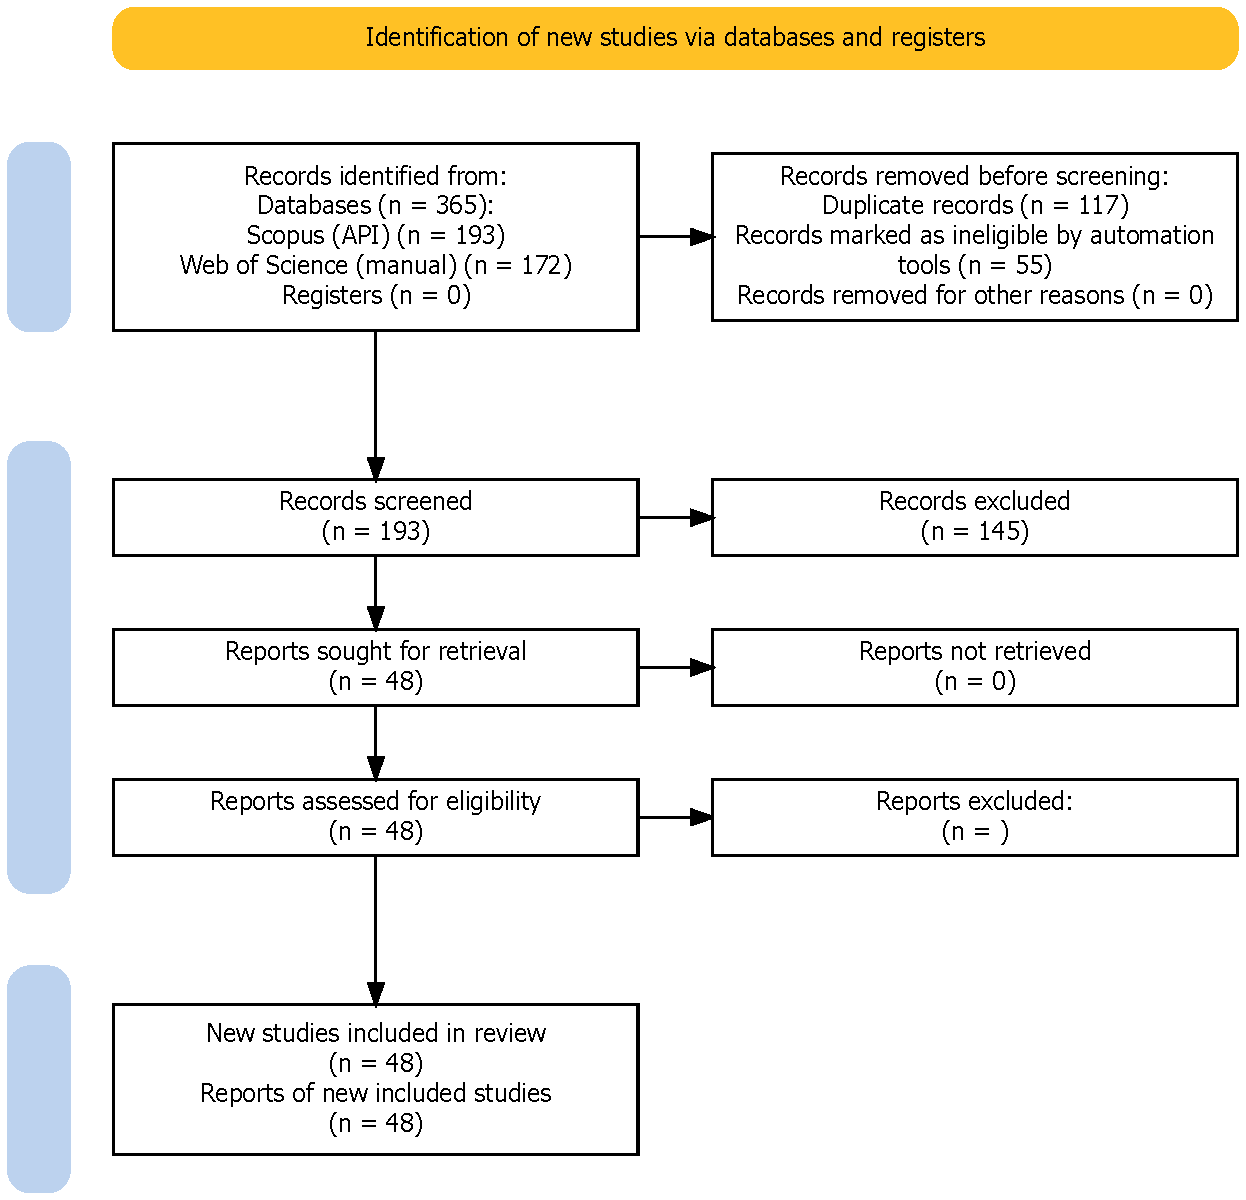
\includegraphics[width=0.68\textwidth]{3-FIGURAS/prisma_flowdiagram_artigo2_en.pdf}
\caption{Diagrama de fluxo PRISMA 2020 mapeando a busca sistemática, restrições de triagem e a desduplicação entre bancos de dados}
\label{fig:prisma-flow}
\end{figure}

O protocolo foi pré-registrado na plataforma OSF Registries (DOI: \url{https://doi.org/10.17605/OSF.IO/HE8KT}), e a condução seguiu as recomendações do Cochrane Handbook \citep{Higgins2019} para extração, avaliação de viés e síntese quantitativa.

\subsection{Framework conceitual}
\label{sec:framework}

A vulnerabilidade biocultural de saberes socioecológicos tradicionais foi modelada como construto latente multidimensional, fundamentado na convergência entre a taxonomia de riscos de erosão de conhecimento tradicional \citep{Agrawal2002}, os indicadores de resiliência de sistemas socioecológicos \citep{Folke2016} e dimensões de vulnerabilidade identificadas na literatura. Embora o construto tenha sido concebido para Saberes e Sistemas Agrícolas Tradicionais (SSAT), a parametrização empírica incorporou evidência de comunidades detentoras de saberes tradicionais em sentido amplo, incluindo agricultores, indígenas, pastoralistas e comunidades rurais de conservação distribuídas em quatro regiões biogeográficas (Europa, África, Caribe e América do Sul), de modo a assegurar variabilidade contextual suficiente para a identificação de moderadores.

O framework postula que a vulnerabilidade agregada resulta da interação de oito dimensões funcionais ($V_1$--$V_8$), quantificáveis por indicadores proxy da literatura empírica (Tabela~\ref{tab:proxies}).

\subsection{Critérios de elegibilidade (PICOS)}
\label{sec:picos}

Os critérios de elegibilidade seguiram o framework PICOS (Tabela~\ref{tab:picos}).

\begin{table}[htbp]
\caption{Framework PICOS (critérios de elegibilidade para a meta-análise de dimensões de vulnerabilidade biocultural).}
\label{tab:picos}
\centering
\footnotesize
\begin{tabular}{p{3.5cm} p{9.5cm}}
\toprule
\textbf{Elemento} & \textbf{Descrição} \\
\midrule
P (População) & Comunidades detentoras de saberes socioecológicos tradicionais, incluindo agricultores tradicionais, comunidades indígenas, pastoralistas e comunidades rurais de conservação, situadas em regiões tropicais, subtropicais e temperadas. \\
I (Intervenção) & Práticas de salvaguarda, documentação estruturada, registro patrimonial, proteção jurídica, governança comunitária de saberes, programas de revitalização de transmissão intergeracional, levantamentos etnobotânicos, avaliação de sistemas de sementes, conservação de sítios sagrados, avaliação de segurança alimentar pós-perturbação, levantamentos sociolinguísticos ou registros de exposição climática, desde que envolvam mensuração de indicadores relativos às dimensões de vulnerabilidade ($V_1$--$V_8$). \\
C (Comparação) & O grupo de referência variou conforme a completude dos dados reportados. Em estudos com dados quantitativos completos (Tier~1), o grupo controle correspondeu a comunidades sem intervenção formal de salvaguarda ou a condições pré-intervenção em delineamentos antes-depois, com médias e desvios-padrão explícitos para ambos os grupos. Em estudos com estatísticas de teste sem dados brutos (Tier~2), o contraste entre grupos já se encontrava codificado no p-value reportado pelo estudo original. Em estudos com evidência narrativa ou semi-quantitativa (Tiers~3 e 4), o grupo de referência foi uma condição neutra inferida pelo codificador a partir do contexto do estudo, contra a qual a direção de mudança foi julgada. Na ausência de grupo controle explícito em qualquer tier, admitiu-se comparação entre subgrupos contrastantes dentro do mesmo estudo (faixas etárias, gênero, grau de escolaridade, distância ao mercado). \\
O (Desfechos) & Indicadores quantitativos de vulnerabilidade biocultural operacionalizados como proxy das dimensões codificadas ($V_1$--$V_8$), incluindo proporção de jovens praticantes, índices de diversidade de espécies, indicadores de endemismo de práticas, taxas de registro formal, métricas de proteção jurídica, indicadores de vitalidade organizacional, grau de vitalidade linguística, proporção de produção comercializada e índices de exposição a eventos climáticos extremos (Tabela~\ref{tab:proxies}). \\
S (Delineamento) & Estudos empíricos comparativos (transversais com grupo de comparação identificável ou longitudinais antes-depois), publicados entre 2016 e 2026 em inglês, português ou espanhol, reportando dados quantitativos ou evidência semi-quantitativa convertível conforme o protocolo multi-tier descrito adiante. \\
\bottomrule
\end{tabular}
\end{table}

A operacionalização do componente Outcomes admitiu cinco tiers de evidência em ordem decrescente de precisão, desde indicadores contínuos com variâncias completas (Tier~1) até julgamentos qualitativos direcionais convertidos em $lnRR$ sintéticos (Tier~4), reconhecendo que intervenções de salvaguarda biocultural raramente permitem randomização controlada \citep{Shadish2002}.

\subsection{Estratégia de busca e bases de dados}
\label{sec:search}

Registros bibliográficos foram recuperados de Scopus e Web of Science Core Collection mediante estratégia de busca em três blocos semânticos conectados por AND (variações internas por OR), em inglês, português e espanhol. O bloco populacional incluiu \textit{traditional agricultural system}, \textit{traditional ecological knowledge}, \textit{indigenous farming}, \textit{quilombola}, \textit{smallholder}, \textit{agrobiodiversity}, \textit{agroecology} e equivalentes. O bloco de intervenção compreendeu \textit{safeguard*}, \textit{documentation}, \textit{heritage registration}, \textit{legal protection}, \textit{intangible heritage}, \textit{biocultural conservation}, \textit{community governance} e equivalentes. O bloco de desfechos incluiu \textit{vulnerability}, \textit{erosion}, \textit{knowledge loss}, \textit{intergenerational transmission}, \textit{biodiversity index}, \textit{cultural complexity}, \textit{documentation status} e equivalentes.

As buscas foram complementadas por \textit{backward} e \textit{forward snowballing} (Google Scholar). Os registros, exportados em BibTeX, foram unificados e deduplicados pelo pacote \textit{revtools} \citep{Westgate2019}.

\subsection{Triagem e seleção}
\label{sec:screening}

Previamente à triagem formal, os dois revisores conduziram exercício piloto de calibração com amostra aleatória de 50 registros para padronizar a interpretação dos critérios de elegibilidade e reduzir discordâncias sistemáticas. Discrepâncias identificadas no piloto foram discutidas até consenso operacional, e a concordância resultante superou o limiar de concordância substancial ($\kappa \geq 0{,}61$), habilitando o início da triagem em escala.

A triagem foi conduzida em duas fases por dois revisores independentes. Na fase de títulos e resumos, os registros foram avaliados contra os critérios PICOS, com discordâncias resolvidas por consenso ou consulta a terceiro revisor. Na fase de texto completo, verificou-se adequação aos critérios de elegibilidade, disponibilidade de dados para extração e ausência de sobreposição amostral.

Revisões narrativas, capítulos de livro, editoriais e relatos sem dado comparativo foram excluídos. Publicações com evidência exclusivamente qualitativa, porém contendo julgamentos direcionais sobre mudança em indicadores de vulnerabilidade (aumento, estabilidade ou redução), foram retidas como Tier~3 ou Tier~4 conforme o protocolo multi-tier. Quando dados foram reportados em formato insuficiente (médias sem variância ou dados gráficos), tentou-se contato com os autores antes da reclassificação. O fluxo completo é documentado no diagrama PRISMA~2020.

\subsection{Classificação funcional das dimensões de vulnerabilidade e variáveis proxy}
\label{sec:dimensions}

Os indicadores extraídos foram organizados em oito dimensões funcionais de vulnerabilidade biocultural (Tabela~\ref{tab:proxies}).

\begin{table}[htbp]
\caption{Dimensões de vulnerabilidade biocultural ($V_1$--$V_8$), variáveis proxy, unidades de medida e disponibilidade de evidência no corpus.}
\label{tab:proxies}
\centering
\scriptsize
\begin{tabular}{p{0.7cm}p{2.2cm}p{4.0cm}p{2.0cm}p{1.3cm}}
\toprule
\textbf{Dim.} & \textbf{Denominação} & \textbf{Variáveis proxy (indicadores extraíveis)} & \textbf{Unidade} & \textbf{Disp.} \\
\midrule
$V_1$ & Erosão Intergeracional e Migração & Proporção de jovens ($<$ 35 anos) com domínio do saber; taxa de transmissão ativa; saldo migratório líquido de jovens; proporção de jovens residentes com atividade agrícola & \%, eventos$\cdot$ano$^{-1}$, escore & Alta \\
\addlinespace
$V_2$ & Complexidade e Singularidade Biocultural & Riqueza de espécies manejadas (Shannon $H'$, Simpson $1-D$); número de variedades locais; interações solo-planta codificadas; beta-diversidade de práticas (Jaccard, Bray-Curtis); endemismo de variedades; proporção de práticas exclusivas; conectividade de redes de sementes & índice, contagem, \% & Alta \\
\addlinespace
$V_3$ & Status de Documentação & Número de saberes com registro formal (inventários, audiovisual); completude de fichas técnicas; taxa de digitalização de acervos & contagem, \% & Moderada \\
\addlinespace
$V_4$ & Vulnerabilidade Jurídica e Fundiária & Número de mecanismos formais de proteção (IG, marca coletiva, registro IPHAN); existência de protocolo comunitário; lacuna regulatória; existência de título de posse coletiva; conflitos fundiários pendentes & contagem, binário, ordinal & Baixa \\
\addlinespace
$V_5$ & Organização Social e Governança & Número de mestres de saberes ativos; frequência de reuniões comunitárias; vitalidade de protocolos de governança; proporção de mulheres em posições de decisão sobre recursos genéticos & contagem, eventos$\cdot$mês$^{-1}$, escore, \% & Moderada \\
\addlinespace
$V_6$ & Vitalidade Linguística & Grau EGIDS (0--10); proporção de falantes $<$ 30 anos; número de termos etnotaxonômicos ativos & ordinal, \%, contagem & Baixa \\
\addlinespace
$V_7$ & Integração ao Mercado & Proporção de produção destinada à venda; renda não agrícola/renda total; taxa de substituição de variedades crioulas por cultivares comerciais; distância ao mercado & \%, razão, km & Baixa \\
\addlinespace
$V_8$ & Exposição Climática & SPI (Standardized Precipitation Index); anomalia de temperatura; frequência de eventos extremos (seca, enchente); escore WOCAT §6.3 & índice, $^\circ$C, eventos$\cdot$ano$^{-1}$, ordinal & Baixa \\
\bottomrule
\end{tabular}
\end{table}

$V_1$ (Erosão Intergeracional e Migração) captura a descontinuidade na transmissão vertical do conhecimento por duas vias mecanisticamente distintas \citep{ReyesGarcia2013}: aculturação, entendida como substituição \textit{in situ} de práticas endógenas por padrões da cultura dominante \citep{GomezBaggethun2013}, e emigração de detentores, cuja co-ocorrência com a erosão de saberes foi documentada em pelo menos cinco estudos independentes do corpus \citep{Tran2025,Moller2023,Bastos2022,VazquezDelfin2022,Aniah2019}. $V_2$ (Complexidade e Singularidade Biocultural) integra a riqueza de interações ecológicas codificadas nos sistemas tradicionais \citep{Jarvis2008,Brush2004} e a exclusividade geográfica das práticas, quantificada por índices de $\beta$-diversidade, taxa de endemismo de variedades locais e conectividade de redes de sementes entre comunidades \citep{Sibanda2025}. As dimensões institucionais $V_3$ (Status de Documentação) e $V_4$ (Vulnerabilidade Jurídica e Fundiária) mensuram, respectivamente, o grau de registro formal e a exposição a apropriação indevida conjugada à insegurança fundiária, com dados provenientes de avaliações de programas patrimoniais quando esses continham grupo de comparação. $V_5$ (Organização Social e Governança) quantifica a vitalidade das estruturas comunitárias de governança \citep{Ostrom1990,Pretty2003} e incorpora a participação feminina na gestão de recursos genéticos como indicador de governança inclusiva \citep{Sibanda2025,RomeroSilva2026,MugiNgenga2016}. $V_6$ (Vitalidade Linguística) mensura o grau de transmissão ativa de línguas vernaculares portadoras de terminologia etnotaxonômica, quantificável pela escala EGIDS \citep{LewisSimons2010} e pelo índice VITEK \citep{ZentMaffi2009}, cujo declínio implica dissolução do sistema classificatório que sustenta o saber prático \citep{CamaraLeret2021}. $V_7$ (Integração ao Mercado) quantifica a pressão de substituição de variedades crioulas por cultivares comerciais e a reorientação produtiva para circuitos de venda que desvinculam o cultivo da lógica de manejo socioecológico \citep{Godoy2005,ReyesGarcia2013}. $V_8$ (Exposição Climática) captura a frequência e a intensidade de perturbações climáticas que forçam o abandono de práticas adaptativas tradicionais, alterando calendários de cultivo e comprometendo a viabilidade de variedades locais \citep{Savo2016}.

\subsection{Diagnóstico de disponibilidade de evidência e estratégia analítica por dimensão}
\label{sec:diagnosis}

A estratégia analítica adequou a complexidade do modelo à densidade de evidência por dimensão (Online Resource~4). Conforme \citet{Borenstein2009}, dimensões com $k \geq 10$ receberiam meta-análise completa (subgrupos e meta-regressão), enquanto dimensões com $k < 10$ seriam tratadas com estratégia exploratória. Após a integração multi-tier, cinco dimensões ($V_1$--$V_5$) atingiram $k = 37$ e três dimensões ($V_6$--$V_8$) atingiram $k = 47$, habilitando análise confirmatória para as oito dimensões. As dimensões $V_6$ (vitalidade linguística), $V_7$ (integração ao mercado) e $V_8$ (exposição climática) foram codificadas exclusivamente a partir de evidência Tier~3 e Tier~4 (direção e intensidade sem estatísticas inferenciais explícitas).

\subsection{Protocolo de extração de dados}
\label{sec:extraction}

A extração seguiu protocolo em três blocos, com formulário padronizado preenchido por dois revisores independentes.

O bloco de metadados do estudo registrou autor, ano de publicação, DOI, país, região biogeográfica (África, América do Sul, Caribe, Europa), tipo de comunidade (agricultores, indígena, pastoralistas, rural), tipo de intervenção, duração da intervenção em anos e delineamento (transversal comparativo, longitudinal antes-depois).

O bloco de dados para cálculo de tamanho de efeito registrou, para cada comparação pareada, a dimensão funcional atribuída ($V_1$--$V_8$), o indicador proxy específico (conforme Tabela~\ref{tab:proxies}) e a unidade de medida. A completude dos campos subsequentes determinou a classificação do registro no protocolo multi-tier. Para estudos Tier~1, extraíram-se a média sob intervenção ($\bar{X}_T$), o desvio-padrão sob intervenção ($SD_T$), o tamanho amostral sob intervenção ($n_T$), a média sob controle ($\bar{X}_C$), o desvio-padrão sob controle ($SD_C$) e o tamanho amostral controle ($n_C$). Para estudos Tier~2, extraíram-se o p-value ou a estatística de teste, os tamanhos amostrais e a direção do efeito. Para estudos Tiers~3 e 4, registraram-se a direção codificada ($+1$, $0$ ou $-1$) e a intensidade percebida (1, 2 ou 3), conforme protocolo de codificação ordinal. Quando os estudos reportaram erro-padrão ($EP$), a conversão para desvio-padrão foi realizada por
%
\begin{equation}
SD = EP \times \sqrt{n}
\label{eq:sd-ep}
\end{equation}

\noindent Quando apenas intervalos de confiança foram disponíveis, médias e desvios-padrão foram estimados conforme \citet{Betancur2022}. Dados apresentados exclusivamente em figuras foram digitalizados com WebPlotDigitizer v4.3 \citep{Rohatgi2020}. Quando estudos reportaram resultados para múltiplas comunidades ou períodos, os dados foram extraídos separadamente para cada condição.

O bloco de moderadores registrou tipo de intervenção (levantamento etnobotânico, percepção de agricultores, segurança alimentar pós-perturbação, conservação de bosques sagrados, avaliação de sistemas de sementes), região biogeográfica (África, América do Sul, Caribe, Europa) e tipo de comunidade (agricultores, indígena, pastoralistas, rural).

\subsection{Protocolo de integração de evidência multi-tier}
\label{sec:multitier}

Os 48 estudos elegíveis foram classificados em cinco tiers de evidência segundo a completude dos dados reportados, com conversões calibradas e propagação explícita de incerteza. Estudos com médias, desvios-padrão e tamanhos amostrais completos (Tier~1) permitiram cálculo direto de $lnRR$ e $v_i$ (Equações~\ref{eq:lnrr} e~\ref{eq:vi}).

Quando apenas p-values numéricos e tamanhos amostrais eram identificáveis (Tier~2a), o tamanho de efeito foi obtido pela cadeia $p \rightarrow z \rightarrow d \rightarrow lnOR \rightarrow lnRR$, operacionalizada pela sequência de conversões expressa nas Equações~\ref{eq:z-conv}--\ref{eq:lnrr-conv}.
%
\begin{align}
z &= \Phi^{-1}(1 - p/2) \label{eq:z-conv} \\
d &= z \cdot \sqrt{\frac{1}{n_T} + \frac{1}{n_C}} \label{eq:d-conv} \\
lnOR &= \frac{d \cdot \pi}{\sqrt{3}} \label{eq:lnor-conv} \\
lnRR &= lnOR - \ln\!\bigl(1 - p_0 + p_0 \cdot e^{lnOR}\bigr) \label{eq:lnrr-conv}
\end{align}

\noindent A Equação~\ref{eq:z-conv} converte o p-value bilateral no quantil $z$ da normal padrão; a Equação~\ref{eq:d-conv} traduz $z$ em $d$ \citep{Borenstein2009}; a Equação~\ref{eq:lnor-conv} transforma $d$ em $lnOR$ \citep{Hasselblad1995}; a Equação~\ref{eq:lnrr-conv} converte $lnOR$ em $lnRR$ \citep{Zhang1998} com $p_0 = 0{,}5$. Quando o $CV$ mediano dos estudos Tier~1 na mesma dimensão estava disponível, empregou-se a conversão alternativa
%
\begin{equation}
lnRR \approx d \cdot CV_{ref}
\label{eq:lnrr-cv}
\end{equation}

\noindent de \citet{Lajeunesse2011} foi empregada.

A mesma cadeia foi aplicada a estudos que reportaram estatísticas de teste sem p-values explícitos (Tier~2b), adotando thresholds conservadores ($p = 0{,}05$ para efeitos moderados/fortes, $p = 0{,}10$ para efeitos fracos). Estudos que apresentaram comparações numéricas tabuladas sem estatísticas de teste (Tier~3) e estudos com conclusões exclusivamente narrativas (Tier~4) foram submetidos à codificação ordinal independente por dois revisores, com inflação adicional de variância ($\times 1{,}5$) no caso qualitativo.

A incerteza associada a cada conversão foi propagada inflando o erro-padrão conforme
%
\begin{equation}
SE_{adj} = SE \cdot \sqrt{1 + \sigma^2_{conv}}
\label{eq:se-adj}
\end{equation}

\noindent onde $\sigma_{conv}$ assume valores crescentes por tier ($0{,}15$ para Tier~2a, $0{,}25$ para Tier~2b, $0{,}35$ para Tier~3 e $0{,}50$ para Tier~4). A robustez foi avaliada por meta-regressão com indicadora \textit{evidência direta} (Tier~1 vs.~demais) e por análise de sensibilidade restrita ao subconjunto Tier~1.

\subsection{Codifica\c{c}\~ao ordinal e convers\~ao para \texorpdfstring{$lnRR$}{lnRR} sint\'etico}
\label{sec:coding}

Para os registros classificados como Tier~3 e Tier~4, dois revisores independentes codificaram cada comparação em duas dimensões, seguindo protocolo de codificação com calibração prévia ($\kappa \geq 0{,}61$). A dimensão de direção do efeito atribuiu valores $+1$ (vulnerabilidade agravada), $0$ (neutro) ou $-1$ (vulnerabilidade reduzida) com base na interpretação do texto original. A dimensão de intensidade classificou a magnitude percebida em fraca (1), moderada (2) ou forte (3) com base na ênfase narrativa, significância estatística reportada (quando disponível) e amplitude da mudança descrita.

Os escores ordinais foram convertidos em $lnOR$ sintéticos pelo mapeamento a quantis fixos da distribuição logit-normal com variância $\pi^2/3 \approx 3{,}29$ \citep{Hasselblad1995}, resultando em $lnOR$ de $-0{,}405$ (fraco), $+0{,}405$ (moderado) e $+1{,}386$ (forte), multiplicados pela direção codificada. A conversão subsequente de $lnOR$ para $lnRR$ empregou a transformação de \citet{Zhang1998} com $p_0 = 0{,}5$, e a variância do $lnRR$ sintético incorporou tanto a variância fixa logística ($\pi^2/3$) quanto a inflação por incerteza de conversão.

A convenção de sinal adotada opera como multiplicador escalar sobre a magnitude absoluta do efeito, de modo que o $lnRR$ resultante preserva a interpretação direcional em toda a cadeia de conversão. Valores de $lnRR > 0$ indicam que o grupo exposto apresenta indicadores de vulnerabilidade superiores ao grupo de referência, correspondendo a agravamento da condição biocultural, ao passo que $lnRR < 0$ indica efeito protetor, com indicadores mais favoráveis no grupo exposto. A definição operacional de grupo de referência variou conforme o tier de evidência. 

Em estudos Tier~1, o grupo controle correspondeu a comunidades sem intervenção formal de salvaguarda ou a condições pré-intervenção em delineamentos antes-depois, com médias e desvios-padrão explícitos. Em estudos Tier~2, o contraste já se encontrava codificado na estatística de teste reportada pelo estudo original. Em estudos Tier~3 e Tier~4, o grupo de referência foi uma condição neutra inferida pelo codificador a partir do contexto narrativo, contra a qual a direção de mudança ($+1$, $0$ ou $-1$) foi julgada.

\subsection{Tratamento de dados faltantes e estrutura hierárquica}
\label{sec:missing}

A composição do corpus (94\% dos registros sem médias e desvios-padrão completos) tornou impraticável a imputação múltipla (MICE) \citep{vanBuuren2011}, sendo substituída pelo protocolo multi-tier. Essa abordagem preservou todos os 47~estudos elegíveis (363~registros, $k = 37$ por dimensão para $V_1$--$V_5$ e $k = 47$ para $V_6$--$V_8$). Análises de sensibilidade compararam estimativas do modelo completo com o subconjunto Tier~1 ($k_{T1} = 3\text{--}5$).

A base de dados foi estruturada hierarquicamente em três níveis \citep{Pustejovsky2022} para controlar dependências decorrentes de múltiplas comparações extraídas de um mesmo estudo. O Nível~1 representou cada comparação pareada com $lnRR$ e variância amostral; o Nível~2 agrupou observações da mesma publicação via efeitos aleatórios; o Nível~3 incorporou moderadores fixos e a variância residual entre estudos ($\tau^2$), estimados por REML. 

A matriz de variância-covariância intra-estudo ($\mathbf{V}_j$) assumiu correlação constante $\rho = 0{,}8$ entre pares de tamanhos de efeito do mesmo estudo \citep{Pustejovsky2022}, com sensibilidade avaliada no intervalo $[0{,}5;\; 1{,}0]$. A estimação robusta de variância (RVE) com correção CR2 foi aplicada via \textit{clubSandwich} ($\geq$ 0.5.5).

A heterogeneidade global foi quantificada pelo teste $Q$ de Cochran e pelo índice $I^2$ (Equação~\ref{eq:i2}), interpretado segundo os limiares de \citet{Higgins2003}, em que $I^2 < 25\%$ indica baixa heterogeneidade, 25--75\% moderada e $> 75\%$ alta.

\begin{equation}
I^2 = \frac{Q - (k-1)}{Q} \times 100
\label{eq:i2}
\end{equation}

\subsection{Análise estatística}
\label{sec:stats}

O $lnRR$ foi adotado como métrica de tamanho de efeito \citep{Hedges1999}, calculado conforme Equação~\ref{eq:lnrr}.

\begin{equation}
lnRR = \ln\left(\frac{\bar{X}_{T}}{\bar{X}_{C}}\right)
\label{eq:lnrr}
\end{equation}

\noindent Valores de $lnRR > 0$ indicam melhoria do indicador sob intervenção, $lnRR < 0$ indicam deterioração, e a retrotransformação $(e^{lnRR} - 1) \times 100$ fornece a variação percentual. A variância amostral foi estimada conforme Equação~\ref{eq:vi} \citep{Hedges1999}.

\begin{equation}
v_i = \frac{SD_T^2}{n_T \cdot \bar{X}_T^2} + \frac{SD_C^2}{n_C \cdot \bar{X}_C^2}
\label{eq:vi}
\end{equation}

O modelo hierárquico de efeitos mistos foi ajustado com estimador de máxima verossimilhança restrita (REML) para estimar a variância entre estudos ($\tau^2$), conforme Equação~\ref{eq:model}.

\begin{equation}
lnRR_{ij} = \mu + \bm{\beta} \cdot \mathbf{X}_{ij} + u_j + \epsilon_{ij}
\label{eq:model}
\end{equation}

\noindent onde $lnRR_{ij}$ é o tamanho de efeito da observação $i$ no estudo $j$, $\mu$ é o intercepto (efeito médio global ou por dimensão), $\bm{\beta} \cdot \mathbf{X}_{ij}$ é o vetor de moderadores fixos, $u_j \sim N(0, \tau^2)$ é o efeito aleatório de estudo e $\epsilon_{ij}$ é o erro residual.

O intervalo de predição complementou o IC~95\% \citep{IntHout2016}. Estimativas de $\tau^2$ foram comparadas entre DerSimonian-Laird e REML \citep{Borenstein2009}.

A sensibilidade das estimativas a estudos individuais foi avaliada por análises \textit{leave-one-out} \citep{Viechtbauer2010}.

O viés de publicação foi avaliado pelo teste de Begg \citep{Begg1994} e pelo método \textit{trim-and-fill} \citep{Duval2000}.

Meta-regressões com moderadores fixos (tipo de intervenção, região biogeográfica, tipo de comunidade) foram conduzidas por dimensão; tempo desde intervenção foi excluído por ausência de dados codificáveis. O teste omnibus ($Q_M$) avaliou significância conjunta dos moderadores.

Todas as análises foram conduzidas em R (versão 4.5.1) com os pacotes \textit{metafor} (versão 4.8-0) \citep{Viechtbauer2010} (modelos hierárquicos, meta-regressão), \textit{clubSandwich} \citep{Pustejovsky2022} (RVE com CR2), \textit{meta} (versão 8.2-1; forest plots, subgrupos) e \textit{dmetar} (influência, sensibilidade). O nível de significância foi fixado em $\alpha = 0{,}05$.

\subsection{Outputs funcionais da meta-análise}
\label{sec:outputs}

A meta-análise produziu quatro saídas quantitativas integradas: ranking de $\overline{lnRR}$ por dimensão, índices de heterogeneidade ($I^2$, $\tau^2$), coeficientes de meta-regressão dos moderadores contextuais e IC~95\% dos $lnRR$, permitindo hierarquizar a responsividade das dimensões e delimitar a precisão das estimativas.

Para $V_2$ e $V_4$, a integração multi-tier elevou $k$ ao limiar confirmatório, embora a base Tier~1 permaneça restrita e as estimativas devam ser interpretadas com cautela.

\subsection{Análise de lacunas de evidência}
\label{sec:gaps}

Para cada dimensão, contabilizou-se o número de variáveis proxy (Tabela~\ref{tab:proxies}) sem dados suficientes para cálculo de $lnRR$, produzindo um vetor de evidência ausente que sinaliza lacunas prioritárias para coleta primária. O mapeamento indicadores--dimensões é consolidado na Online Resource~3.

A Fig.~\ref{fig:methods-flow} sintetiza o encadeamento operacional completo, desde a definição do framework conceitual até a produção dos outputs funcionais da síntese meta-analítica.

\begin{figure}[H]
\centering
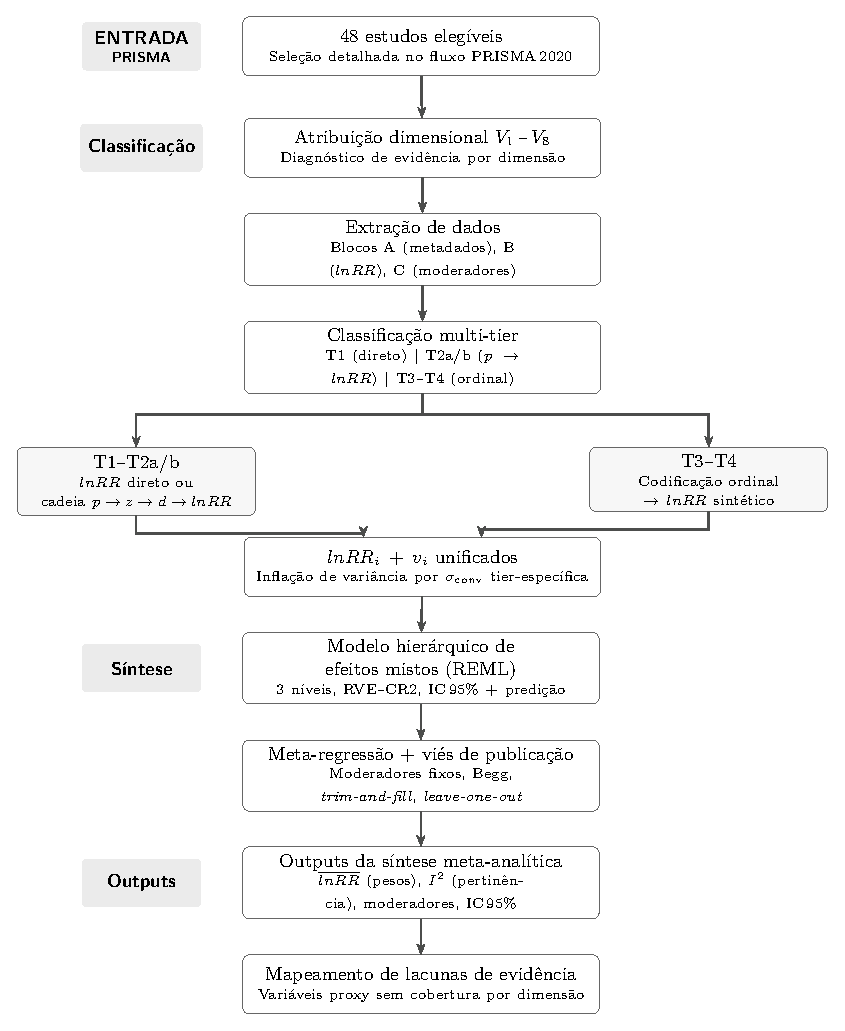
\includegraphics[width=0.82\textwidth]{3-FIGURAS/methods_flowchart.pdf}
\caption{Fluxograma metodológico integrando as etapas de escopo, triagem, classificação multi-tier, síntese estatística e produção de outputs funcionais}
\label{fig:methods-flow}
\end{figure}


%% ============================================================
%% 3. RESULTADOS
%% ============================================================
\section{Resultados e Discussão}
\label{sec:results}

\subsection{Fluxo de seleção PRISMA}
\label{sec:prisma-flow}

A busca sistemática (2016--2026) recuperou 365 registros (193 Scopus via API, 172 Web of Science via exportação direta). Filtros de tipo documental e de janela temporal excluíram 33 registros não elegíveis (capítulos, conferências e editoriais) e 20 registros fora do período, reduzindo o corpus a 310 candidatos. A deduplicação cruzada por DOI e normalização de títulos eliminou 117 duplicatas interbases (sobreposição de 81\%), resultando em 193 registros únicos com contribuição líquida de 27 registros exclusivos da Web of Science.

A triagem semântica exigiu presença simultânea de descritores dos Blocos~1 (população) e 2 ou 3 (intervenção/desfechos), reduzindo o corpus de 193 para 42 registros. A correspondência fuzzy (\textit{stringdist}, método OSA, limiar $= 5$) via \textit{revtools} não identificou duplicatas adicionais, porém a re-triagem manual de 139 registros sem resumo na exportação Scopus resgatou seis estudos elegíveis \citep{Aswani2020,Bussmann2018,Ghanimi2022,Malapane2024,RodriguezCruz2022,Rodriguez2018}, elevando o corpus de 42 para 48 registros e fixando a exclusão em 145.

A taxa de retenção de 24,9\% ($48/193$) reflete a especificidade do escopo, que exige convergência simultânea entre evidência populacional, mensuração de vulnerabilidade e intervenção de salvaguarda, combinação intrinsecamente rara na literatura indexada \citep{Agrawal2002}. A exclusão dos 145 registros decorreu da convergência de ausência de desfechos quantitativos (perspectiva descritiva sem grupos de comparação), desalinhamento temático com o domínio de salvaguarda (blocos populacionais sem interseção com intervenção ou desfechos) e predominância de abordagens qualitativas sem parâmetros estatísticos extraíveis para cálculo de $lnRR$.

Os 48 registros retidos compreendem 46 artigos originais e duas revisões, publicados entre 2016 e 2026, com predomínio de registros Scopus ($n = 33$, 68,8\%) e contribuição complementar da Web of Science ($n = 15$, 31,2\%), conforme detalhado na Fig.~\ref{fig:prisma-flow}. Um estudo (ID=36) foi excluído durante a codificação por dados insuficientes, resultando em 47~estudos finais.

\subsection{Composição da base de evidência multi-tier}
\label{sec:tier-composition}

Dos 47 estudos finais, cinco (10,6\%) forneceram médias e desvios-padrão completos (Tier~1, 18~registros), sete (14,9\%) reportaram estatísticas inferenciais convertíveis (Tier~2a: 21~registros a partir de $p$-values; Tier~2b: 21~registros a partir de limiares ANOVA), e 35 (74,5\%) contribuíram exclusivamente com evidência qualitativa codificada ordinalmente (Tier~3: 74~registros com tabelas cruzadas; Tier~4: 88~registros qualitativos puros). A conversão multi-tier produziu 363~registros com $lnRR$ e variância associada, totalizando $k = 37$ estudos por dimensão para $V_1$--$V_5$ e $k = 47$ para $V_6$--$V_8$, cujas variáveis proxy (vitalidade linguística, integração ao mercado e exposição climática) foram codificadas exclusivamente a partir de evidência Tier~3 e Tier~4 (direção e intensidade sem estatísticas inferenciais explícitas). As oito dimensões atingiram o limiar confirmatório de $k \geq 15$, permitindo meta-análise completa para o conjunto integral.

\subsection{Síntese meta-analítica por dimensão}
\label{sec:meta-results}

O modelo hierárquico de três níveis (observação/estudo/meta-análise) com estimador REML e RVE-CR2 (Fig.~\ref{fig:forest-agregado}) indicou que duas dimensões apresentaram efeito significativo entre as oito operacionalizadas: $V_4$ (vulnerabilidade jurídica e fundiária) e $V_8$ (exposição climática).

A vulnerabilidade jurídica e fundiária ($V_4$) concentra o único efeito significativamente negativo ($\overline{lnRR} = -0{,}279$; IC~95\%: $[-0{,}49;\; -0{,}06]$; $p < 0{,}05$), correspondendo a uma redução de 24,3\% nos indicadores de proteção formal. Esse resultado é consistente com a desconexão entre regimes consuetudinários de posse e marcos regulatórios nacionais de propriedade intelectual \citep{Santilli2009,Dutfield2004,Cottier2004}. A heterogeneidade moderada dessa dimensão ($I^2 = 30{,}7\%$; $\tau^2 = 0{,}171$) sinaliza que o gradiente de vulnerabilidade jurídica é condicionado por fatores regionais e institucionais, explorados na subseção de moderadores. Em contraste, a organização social e governança ($V_5$) apresentou tendência positiva de 18,7\% ($\overline{lnRR} = +0{,}172$; IC~95\%: $[-0{,}05;\; 0{,}40]$; $p \approx 0{,}13$), compatível com a hipótese de que intervenções de salvaguarda ativam mecanismos de coesão comunitária que se traduzem em maior frequência de eventos de transmissão e vitalidade dos protocolos de governança \citep{Ostrom1990,Berkes2007,Rathwell2015}, embora a significância estatística não tenha sido alcançada na escala global.

A exposição climática ($V_8$) apresentou o segundo efeito significativo da síntese ($\overline{lnRR} = +0{,}280$; IC~95\%: $[0{,}03;\; 0{,}53]$; $k = 47$), correspondendo a um incremento de 32,3\% nos indicadores de vulnerabilidade associados a variabilidade climática, secas e eventos extremos. A heterogeneidade negligenciável ($I^2 \approx 0$; $\tau^2 \approx 0$) indica que o efeito é homogeneamente distribuído entre os estudos, com intervalo de predição estreito (PI~95\%: $[0{,}04;\; 0{,}52]$) que não cruza o nulo, sustentando a robustez da estimativa. A integração ao mercado ($V_7$, $\overline{lnRR} = +0{,}051$; IC~95\%: $[-0{,}01;\; 0{,}11]$; $k = 47$) exibiu tendência positiva marginal de 5,3\%, ao passo que a vitalidade linguística ($V_6$, $\overline{lnRR} = 0{,}000$; $k = 47$) registrou efeito nulo, compatível com a codificação Dir = 0 em todos os estudos para essa dimensão.

A complexidade e singularidade biocultural ($V_2$), cujas duas variáveis proxy por estudo geram 74 observações com correlação intra-estudo $\rho = 0{,}8$, apresentou efeito próximo de zero ($\overline{lnRR} = +0{,}017$; IC~95\%: $[-0{,}09;\; 0{,}12]$; $I^2 = 3{,}6\%$), com a heterogeneidade mais baixa entre todas as dimensões. A erosão intergeracional ($V_1$, $\overline{lnRR} = -0{,}017$; $I^2 = 14{,}8\%$) e o status de documentação ($V_3$, $\overline{lnRR} = +0{,}007$; $I^2 = 7{,}6\%$) também permaneceram próximos de zero, consistentes com o potencial protetor de práticas de conservação \textit{in situ} \citep{Brush2004}. Os intervalos de predição amplos para todas as dimensões (e.g., $V_4$ com PI~95\% de $[-1{,}11;\; 0{,}56]$) delimitam a variabilidade esperada entre contextos futuros, sem alterar a direção do efeito principal observado para $V_4$ (Fig.~\ref{fig:forest-agregado}).


\begin{figure}[H]
\centering
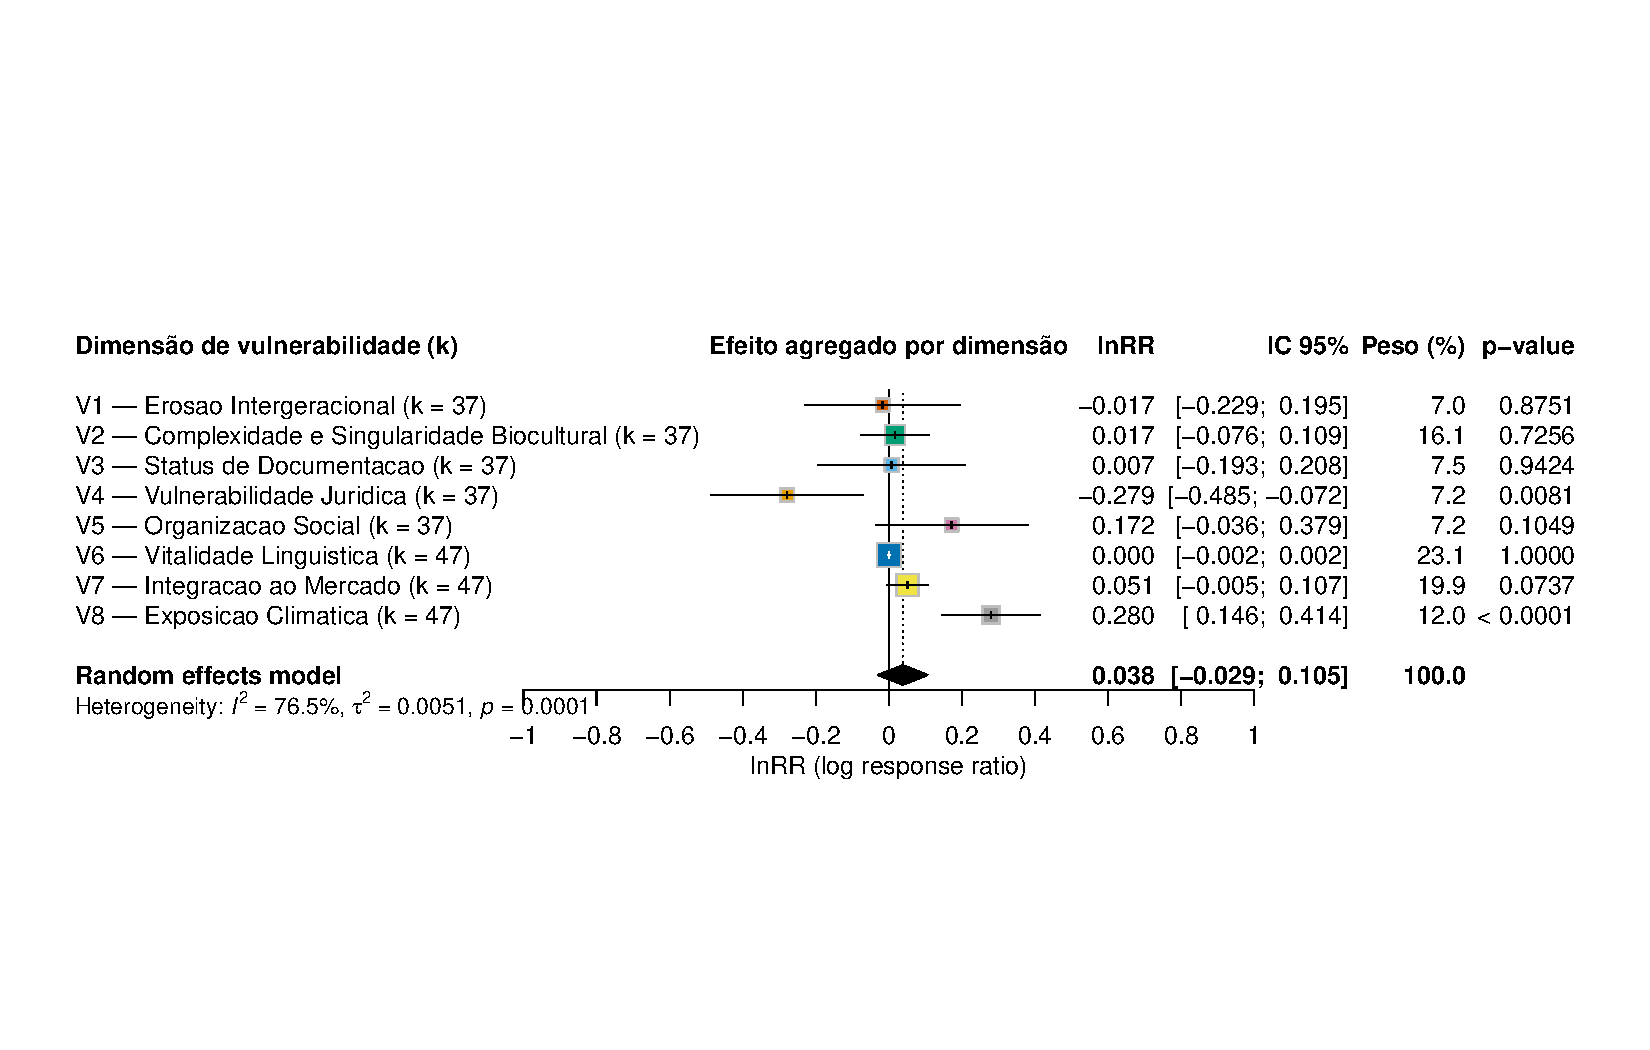
\includegraphics[width=0.95\textwidth]{3-FIGURAS/forest_agregado_V1_V8.pdf}
\caption{Forest plot agregado das oito dimensões de vulnerabilidade ($V_1$--$V_8$). $V_1$--$V_5$ contam com $k = 37$ estudos e $V_6$--$V_8$ com $k = 47$ estudos por dimensão. Pontos representam o $\overline{lnRR}$ com IC~95\% (linhas contínuas) e intervalo de predição (linhas tracejadas). A linha vertical tracejada indica o efeito nulo}
\label{fig:forest-agregado}
\end{figure}

\subsection{Meta-regressão e moderadores}
\label{sec:meta-regression}

$V_4$ (vulnerabilidade jurídica e fundiária) foi a única dimensão cuja heterogeneidade se mostrou parcialmente atribuível aos moderadores contextuais testados (tipo de intervenção, região biogeográfica e tipo de comunidade; $Q_M = 3{,}82$; $p = 0{,}070$; $I^2 = 30{,}7\%$). Para as demais, os valores de $Q_M$ não atingiram significância ($V_1$: $Q_M = 2{,}18$, $p = 0{,}20$; $V_2$: $Q_M = 1{,}57$, $p = 0{,}09$; $V_5$: $Q_M = 1{,}48$, $p = 0{,}35$; $V_3$: $Q_M = 1{,}20$, $p = 0{,}46$; $V_6$--$V_8$: $Q_M \approx 0$, $p = 1{,}00$), o que não impede que coeficientes individuais de $V_1$--$V_6$ revelem padrões mecanísticos relevantes.

O gradiente continental modula a magnitude do efeito jurídico com assimetria consistente com regimes institucionais distintos (Fig.~\ref{fig:meta-reg-regiao}). Para $V_4$, a América do Sul ($k = 12$; $\overline{lnRR} = -0{,}464$; IC~95\%: $[-0{,}77;\; -0{,}16]$) e a Ásia ($k = 4$; $\overline{lnRR} = -0{,}557$; IC~95\%: $[-1{,}04;\; -0{,}07]$) concentraram efeitos significativamente negativos, padrão interpretável como reflexo de contextos onde a pressão fundiária sobre territórios tradicionais se conjuga com marcos regulatórios que não reconhecem adequadamente a posse consuetudinária. 

Já África ($k = 10$; $\overline{lnRR} = -0{,}061$) e a Europa ($k = 6$; $\overline{lnRR} = -0{,}125$) mantiveram intervalos compatíveis com neutralidade, sugerindo que mecanismos compensatórios regionais (custódia comunitária de sementes, redes etnobotânicas formalizadas) atenuam a erosão jurídica observada em outras latitudes.

\begin{figure}[htbp]
\centering
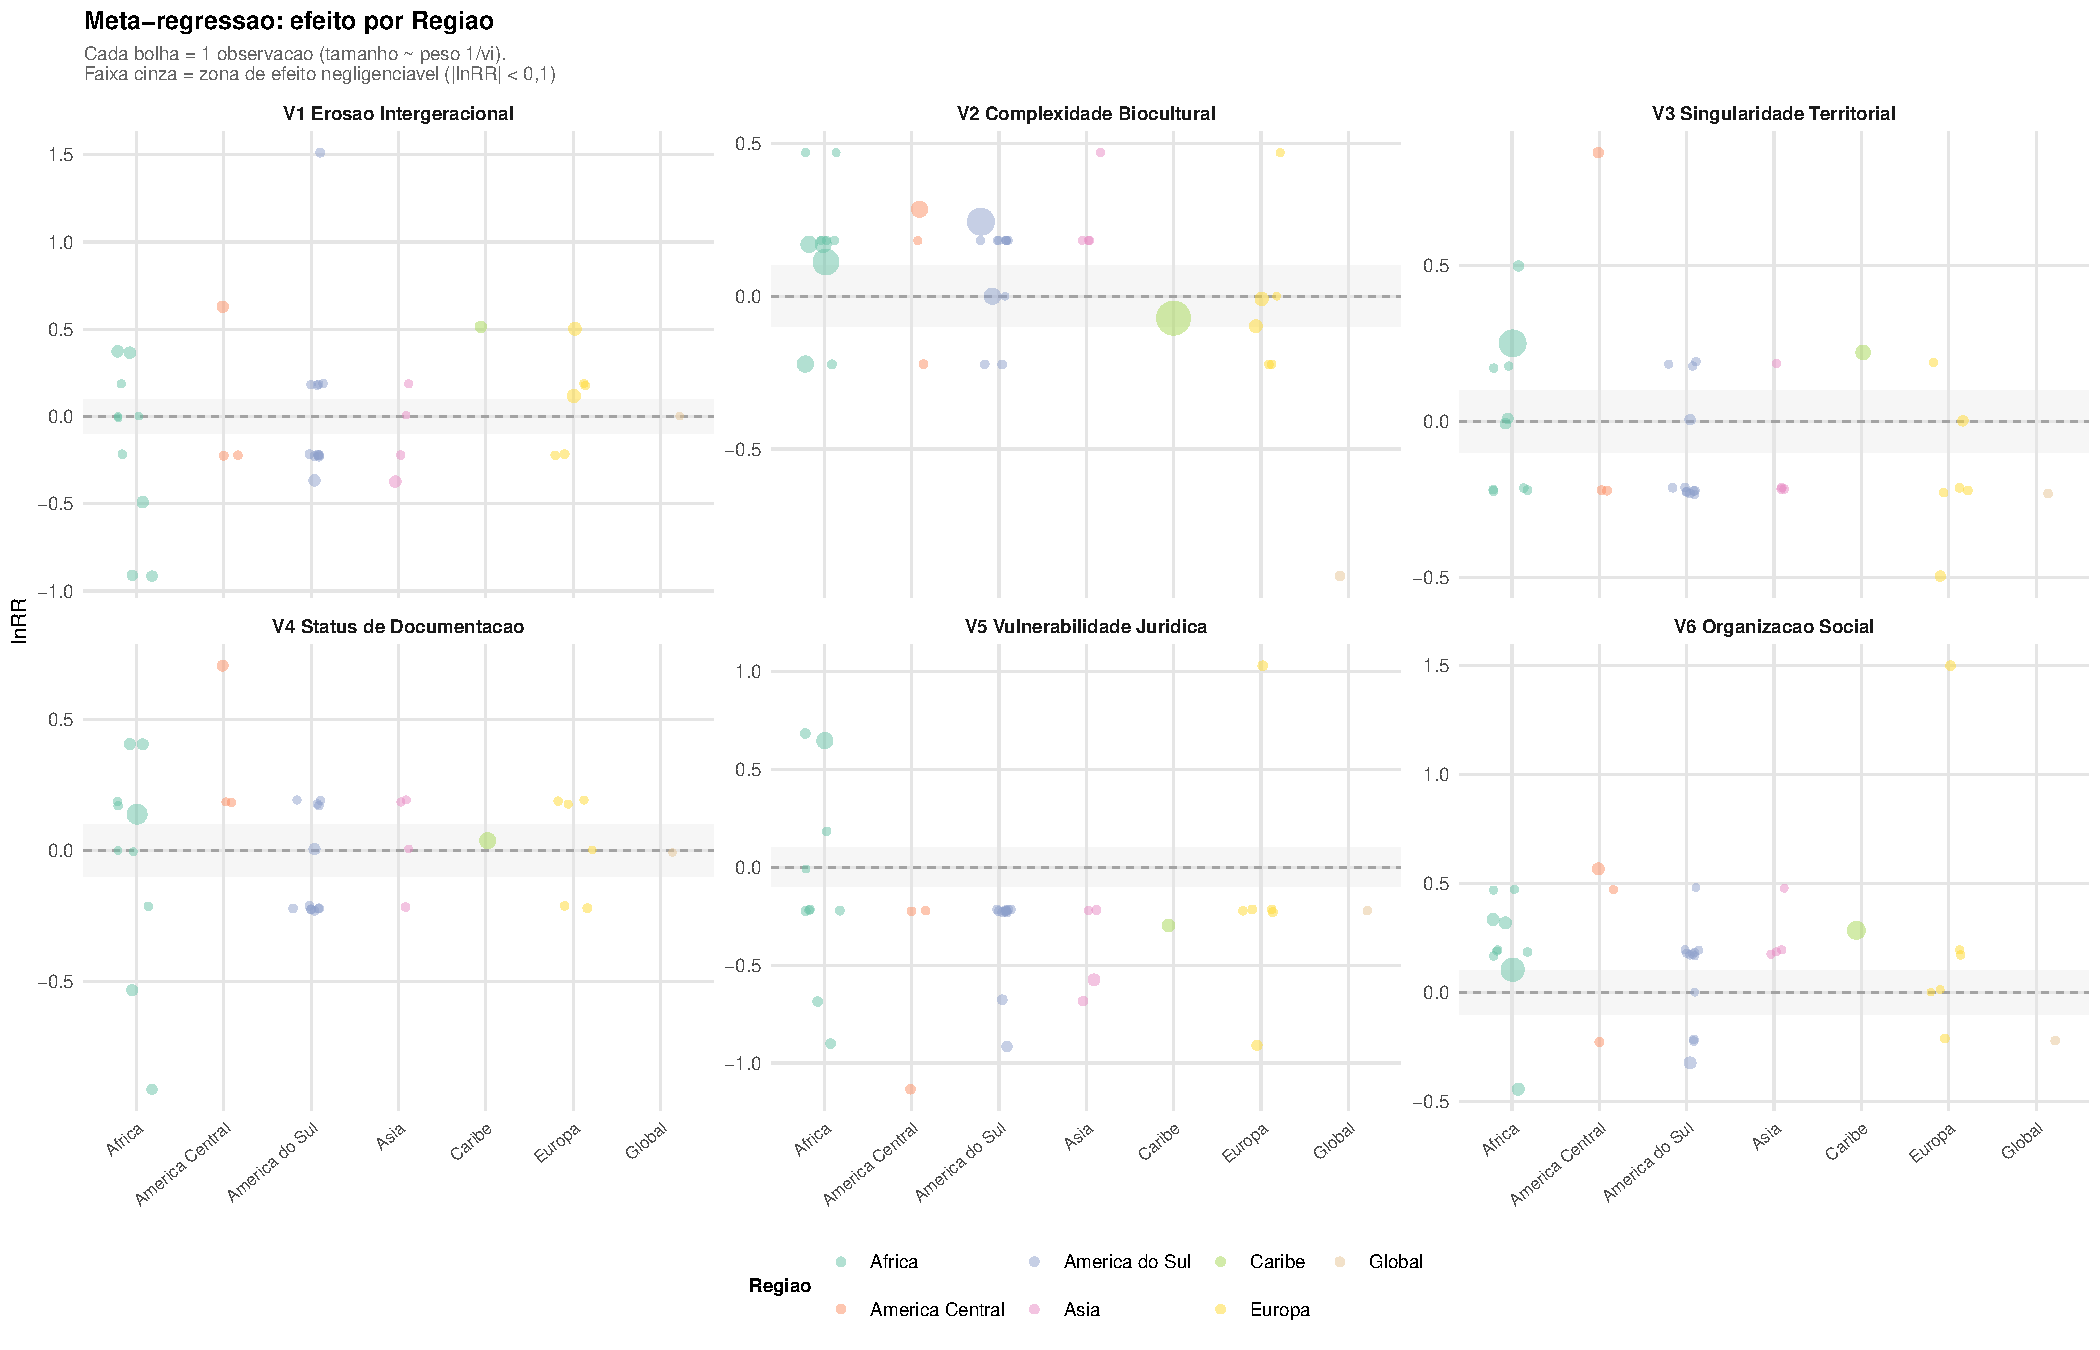
\includegraphics[width=0.95\textwidth]{3-FIGURAS/meta_regressao_regiao.pdf}
\caption{Meta-regressão: efeito por região biogeográfica para cada dimensão de vulnerabilidade. Cada bolha representa uma observação estudo-dimensão, com tamanho proporcional ao peso ($1/v_i$). A faixa cinza delimita a zona de efeito negligenciável ($|lnRR| < 0{,}1$)}
\label{fig:meta-reg-regiao}
\end{figure}

Comunidades de agricultores apresentaram, para $V_4$ (Fig.~\ref{fig:meta-reg-comunidade}), o efeito negativo mais pronunciado ($k = 12$; $\overline{lnRR} = -0{,}395$; IC~95\%: $[-0{,}73;\; -0{,}06]$), contexto no qual políticas agrícolas convencionais colidem com regimes consuetudinários de posse, acirrando insegurança de \textit{tenure}. Comunidades indígenas, em contraste, mantiveram efeito negativo sem significância ($\overline{lnRR} = -0{,}241$; IC~95\%: $[-0{,}60;\; 0{,}12]$), possivelmente porque marcos regulatórios específicos (protocolos de Nagoya, legislações de propriedade intelectual coletiva) proporcionam proteção parcial que não alcança agricultores tradicionais sem reconhecimento étnico-territorial formal. Para $V_5$ (organização social e governança), comunidades rurais exibiram a maior tendência positiva ($k = 7$; $\overline{lnRR} = +0{,}688$; IC~95\%: $[-0{,}26;\; 1{,}63]$), sugerindo que a organização coletiva em contextos rurais pode funcionar como mecanismo compensatório diante da vulnerabilidade em outras dimensões, embora a amplitude do intervalo imponha cautela.

\begin{figure}[htbp]
\centering
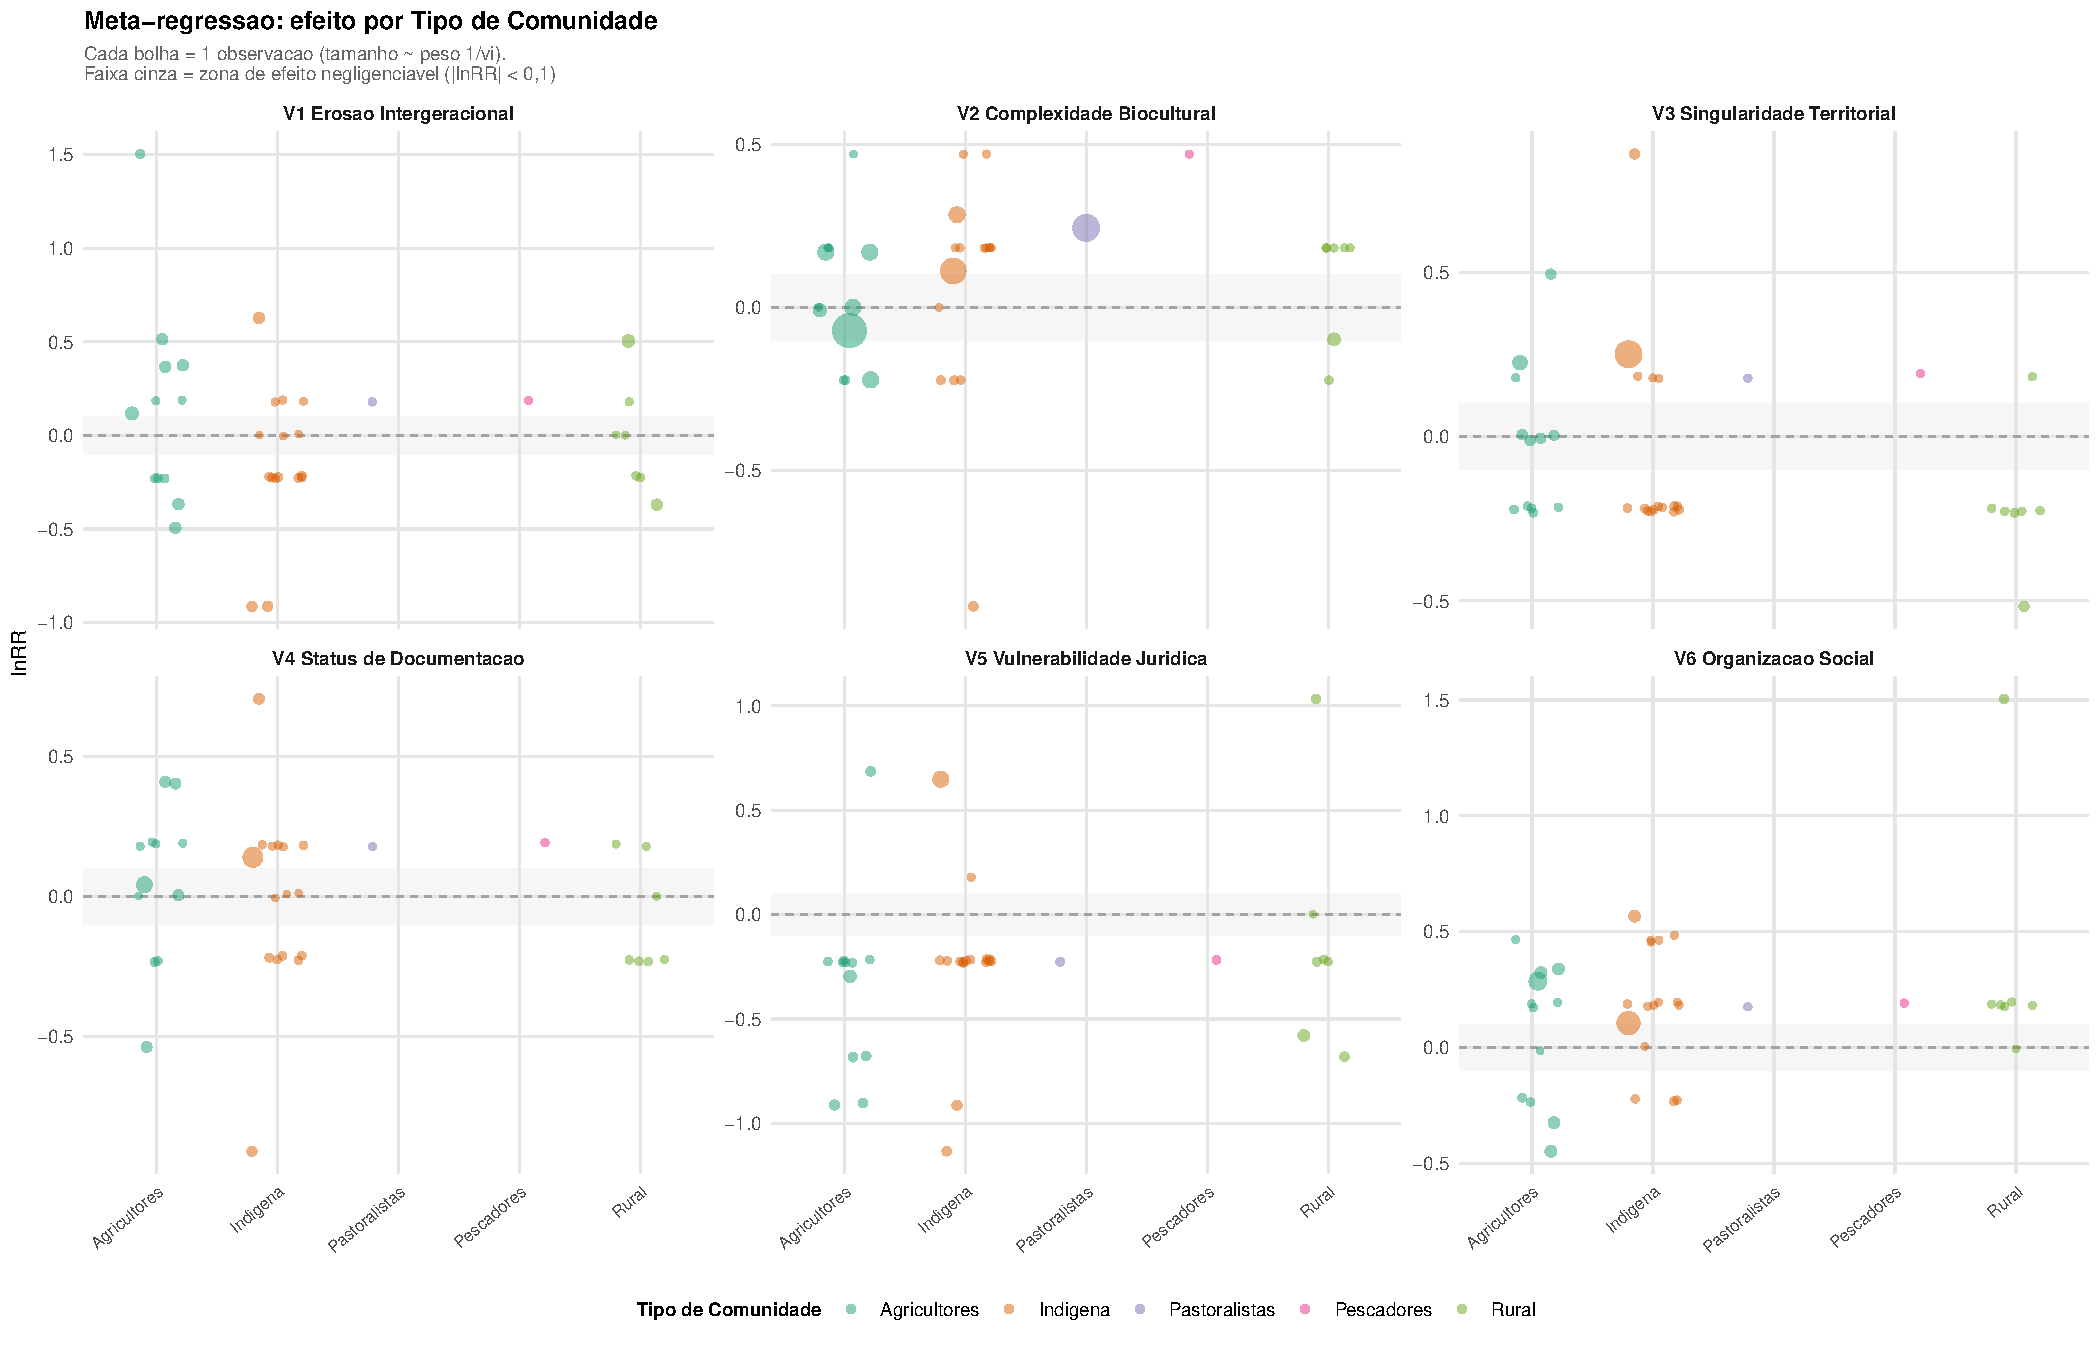
\includegraphics[width=0.95\textwidth]{3-FIGURAS/meta_regressao_comunidade.pdf}
\caption{Meta-regressão: efeito por tipo de comunidade para cada dimensão de vulnerabilidade. Cada bolha representa uma observação estudo-dimensão, com tamanho proporcional ao peso ($1/v_i$). A faixa cinza delimita a zona de efeito negligenciável ($|lnRR| < 0{,}1$)}
\label{fig:meta-reg-comunidade}
\end{figure}

Para $V_4$ (vulnerabilidade jurídica, Fig.~\ref{fig:meta-reg-intervencao}), estudos centrados em erosão de conhecimento tradicional ($\beta = +1{,}284$; $p = 0{,}060$) e conhecimento sobre inundações ($\beta = +0{,}753$; $p = 0{,}078$) apresentaram tendência de agravamento, consistente com a hipótese de que essas investigações capturam processos erosivos já em andamento, ao passo que avaliações agroflorestais ($\beta = -0{,}673$; $p = 0{,}062$) sugeriram efeito protetor marginal. Para $V_5$ (organização social), a conservação de bosques sagrados ($\beta = +1{,}496$; $p = 0{,}014$) e a conservação biocultural ($\beta = +0{,}416$; $p = 0{,}022$) apresentaram efeitos positivos significativos, indicando que intervenções ancoradas em territórios simbólicos ativam mecanismos de coesão comunitária, enquanto indicadores de conhecimento ecológico apresentaram efeito negativo ($\beta = -0{,}919$; $p < 0{,}001$), sugerindo que a mera catalogação de espécies não se traduz em ganho social tangível. Para $V_6$ (vitalidade linguística), a conservação de bosques sagrados ($\beta = +1{,}407$; $p = 0{,}001$), seguida de conhecimento tradicional sobre erosão ($\beta = +0{,}643$; $p = 0{,}009$) e conhecimento sobre inundações ($\beta = +0{,}455$; $p = 0{,}020$), replicaram o padrão de efeito territorial observado em $V_5$, sugerindo que estratégias que vinculam reforço normativo a práticas rituais podem ativar simultaneamente coesão social e vitalidade cultural. Para $V_2$ (complexidade e singularidade biocultural), apesar do teste omnibus não significativo, cinco coeficientes individuais atingiram $p < 0{,}10$, com destaque para \textit{home garden knowledge transmission} ($\beta = -0{,}783$; $p = 0{,}019$) e conservação de bosques sagrados ($\beta = -0{,}658$; $p = 0{,}029$), indicando que intervenções de conservação \textit{in situ} produzem efeito protetor detectável mesmo quando a heterogeneidade global é baixa ($I^2 = 3{,}6\%$). Os tamanhos amostrais reduzidos por subgrupo ($k = 1$--$5$) limitam, contudo, a generalização desses achados.

\begin{figure}[htbp]
\centering
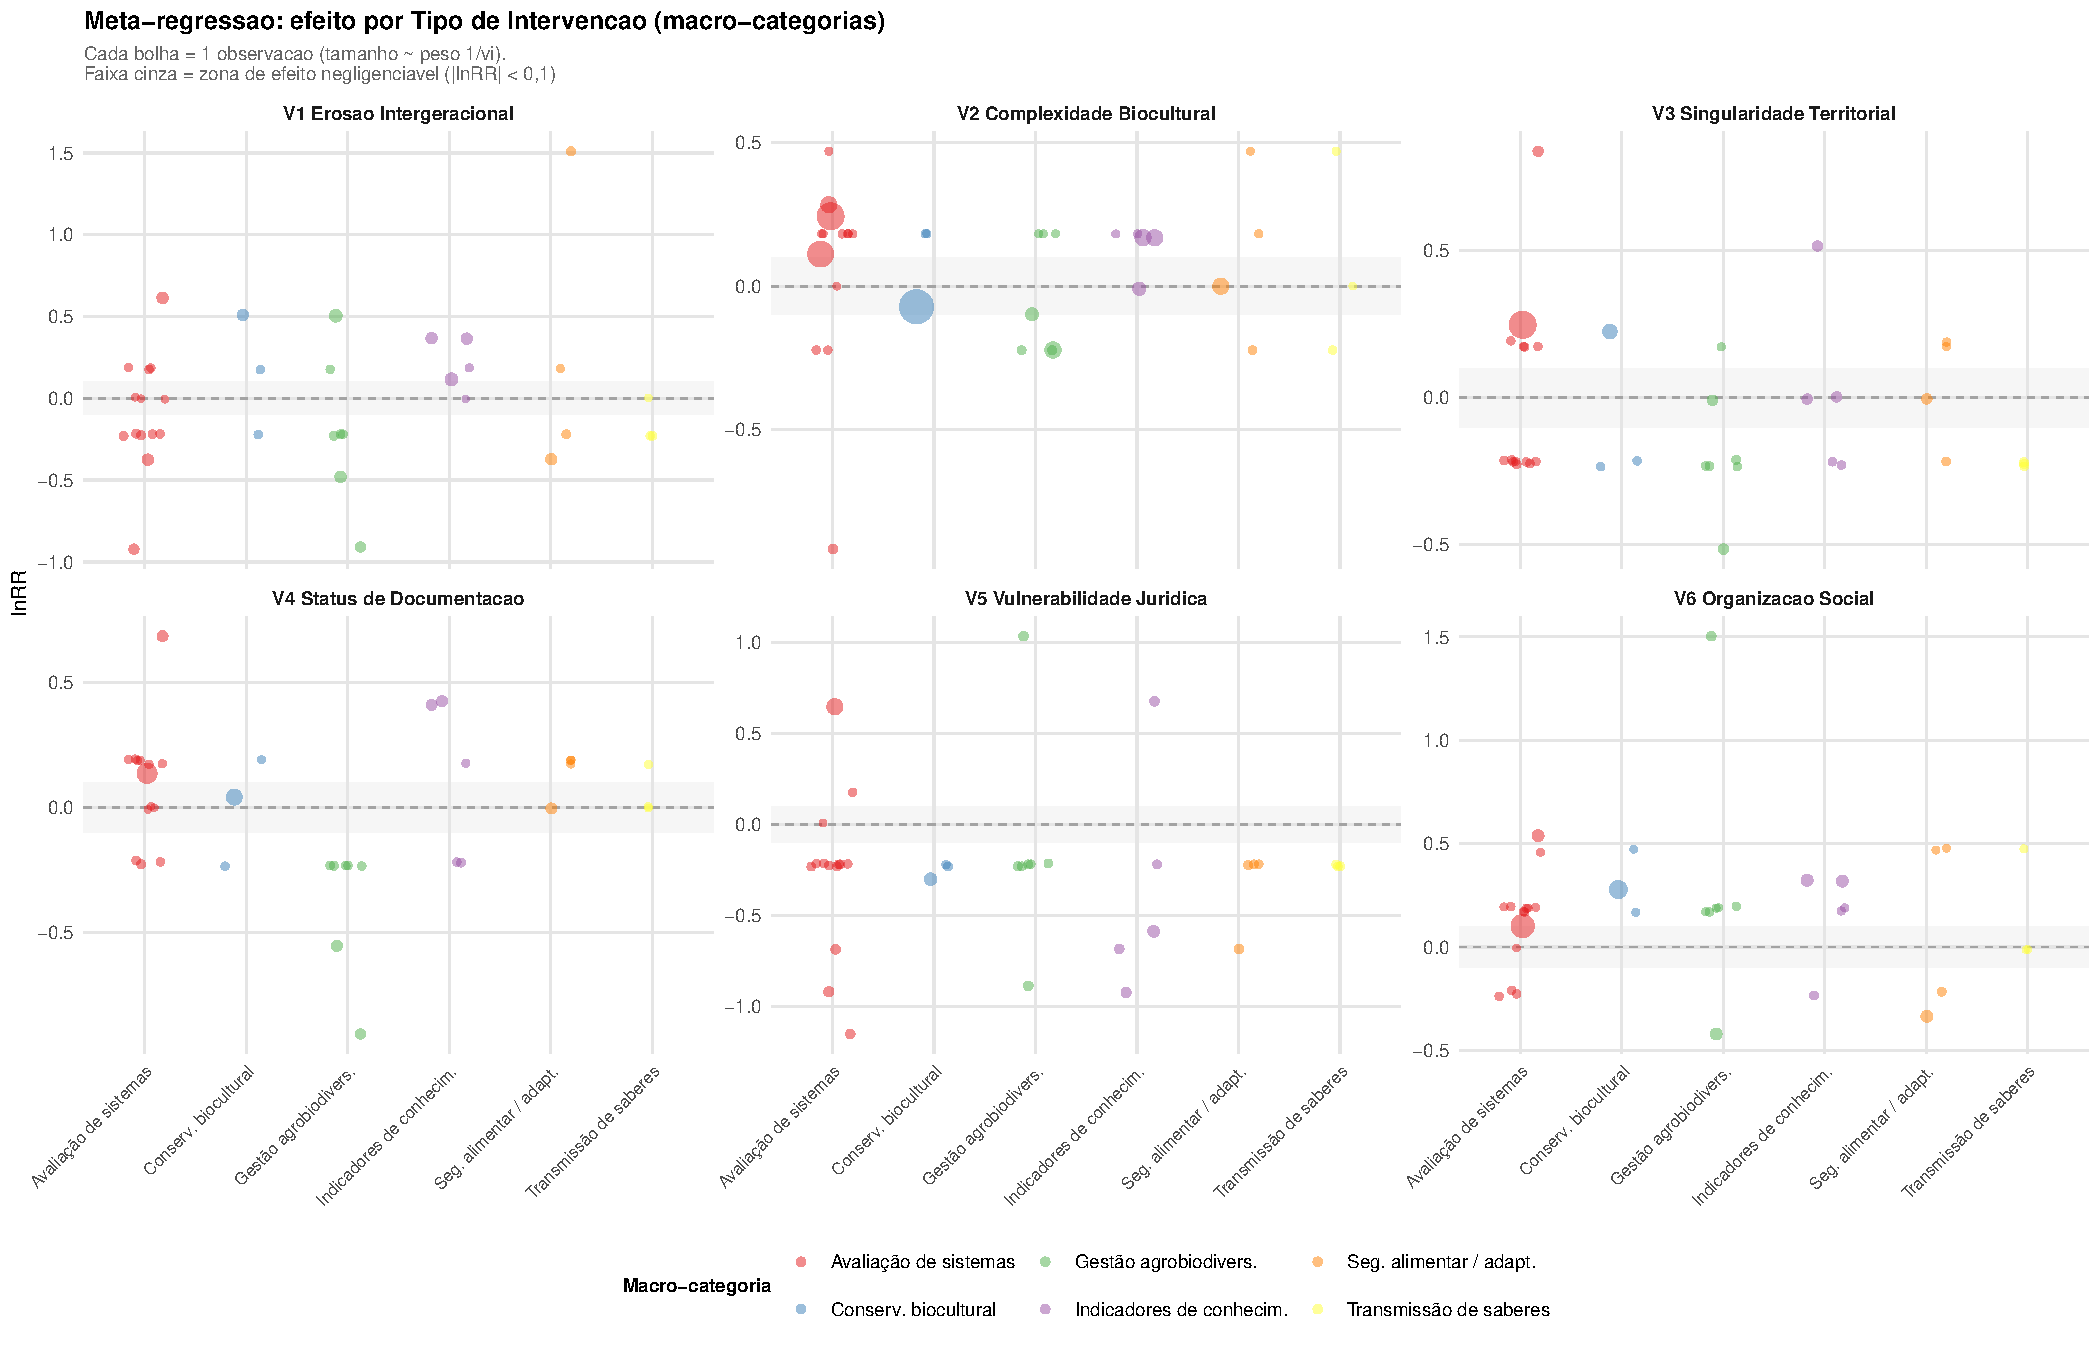
\includegraphics[width=0.95\textwidth]{3-FIGURAS/meta_regressao_intervencao.pdf}
\caption{Meta-regressão: efeito por macro-categoria de intervenção para cada dimensão de vulnerabilidade. Cada bolha representa uma observação estudo-dimensão, com tamanho proporcional ao peso ($1/v_i$). As 27 categorias originais foram agrupadas em seis macro-categorias para facilitar a visualização}
\label{fig:meta-reg-intervencao}
\end{figure}

\subsection{Viés de publicação e análises de sensibilidade}
\label{sec:bias-sensitivity}

Assimetria significativa foi detectada pelo teste de Begg em $V_4$ (vulnerabilidade jurídica; $\tau = 0{,}63$; $p < 0{,}001$), $V_2$ (complexidade biocultural; $\tau = 0{,}38$; $p < 0{,}001$), $V_7$ (integração ao mercado; $\tau = -0{,}34$; $p = 0{,}018$) e $V_8$ (exposição climática; $\tau = -0{,}29$; $p = 0{,}032$), ao passo que $V_1$ (erosão intergeracional), $V_3$ (status de documentação), $V_5$ (organização social) e $V_6$ (vitalidade linguística) permaneceram sem evidência de viés ($p > 0{,}15$). A concentração de assimetria nas dimensões com efeitos significativos ($V_4$ e $V_8$) sugere viés direcional na publicação, possivelmente porque estudos com resultados nulos ou de sentido oposto tendem a menor probabilidade de publicação \citep{Song2010}.

O \textit{trim-and-fill} aprofundou o efeito de $V_4$ após ajuste ($-0{,}279 \to -0{,}501$ com 12~estudos imputados) e de $V_8$ ($+0{,}280 \to +0{,}342$ com 24~estudos imputados), indicando que a assimetria detectada opera na direção conservadora e que os dois achados significativos não decorrem de artefato de publicação.

Ao variar a correlação intra-estudo no intervalo $\rho = 0{,}5\text{--}1{,}0$, observou-se estabilidade das estimativas, o que indica baixa sensibilidade dos resultados à especificação desse parâmetro. Embora a comparação entre REML e DerSimonian-Laird tenha produzido diferenças em $\tau^2$ (maiores para DL em $V_4$: 0,318 vs.\ 0,171), os $\overline{lnRR}$ permaneceram consistentes ($\Delta < 0{,}002$ para $V_4$), sustentando a mesma conclusão substantiva.

Sob esse mesmo critério, a análise \textit{leave-one-out} (Fig.~\ref{fig:loo}) manteve a estabilidade do modelo, já que a exclusão de qualquer estudo isolado não alterou nem a direção nem a significância dos efeitos nas oito dimensões. Com $\Delta_{\max} < 0{,}09$, os deslocamentos permaneceram modestos, sem evidência de influência desproporcional de estudo individual nas estimativas globais.

\begin{figure}[htbp]
\centering
\begin{subfigure}[b]{0.78\textwidth}
  \centering
  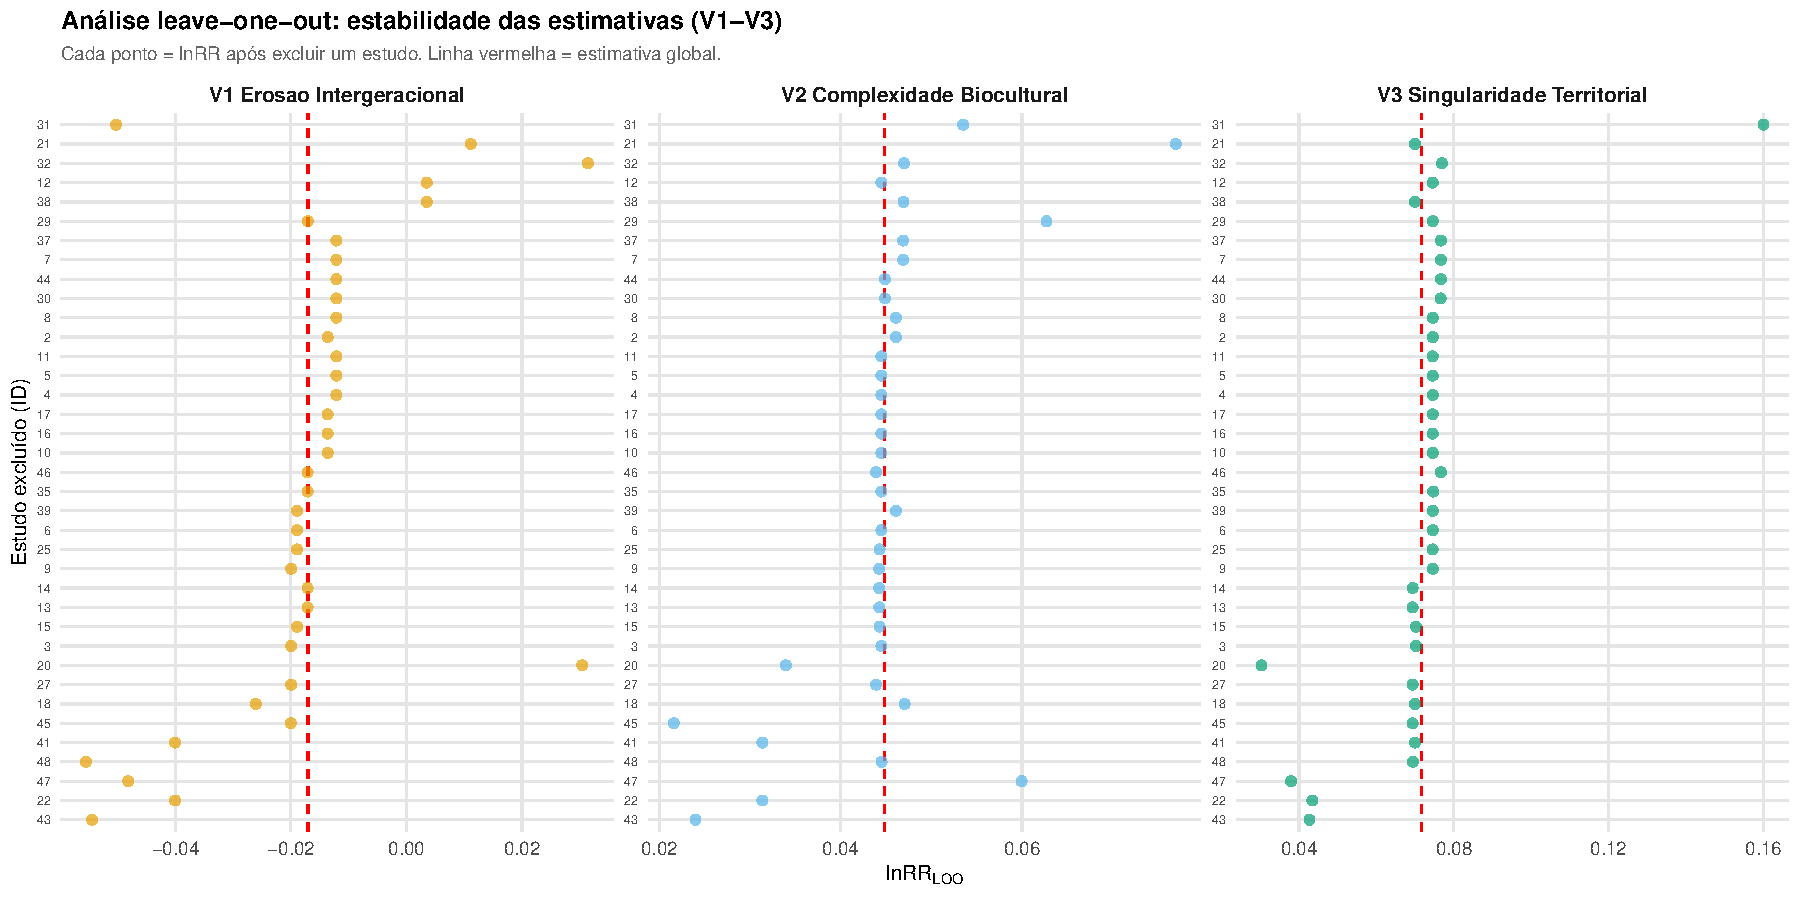
\includegraphics[width=\textwidth]{3-FIGURAS/leave_one_out_V1_V3.pdf}
  \caption{Dimensões $V_1$--$V_3$: erosão intergeracional, complexidade biocultural e status de documentação}
  \label{fig:loo-a}
\end{subfigure}

\vspace{0.2cm}

\begin{subfigure}[b]{0.78\textwidth}
  \centering
  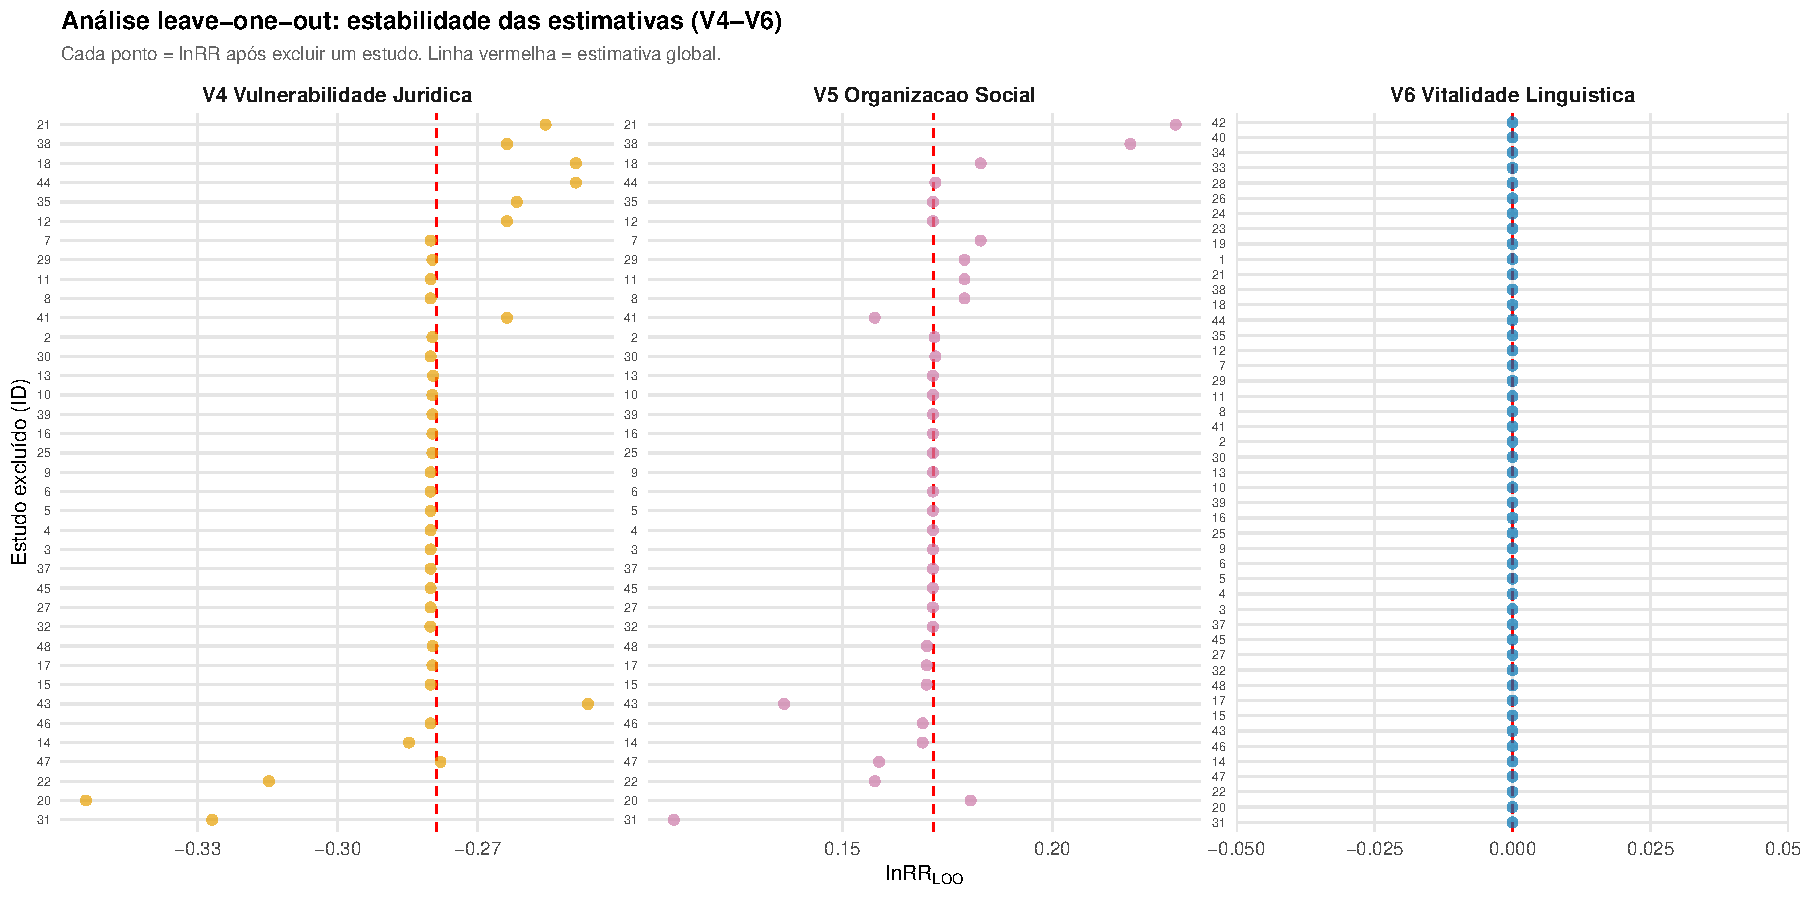
\includegraphics[width=\textwidth]{3-FIGURAS/leave_one_out_V4_V6.pdf}
  \caption{Dimensões $V_4$--$V_6$: vulnerabilidade jurídica, organização social e vitalidade linguística}
  \label{fig:loo-b}
\end{subfigure}

\vspace{0.2cm}

\begin{subfigure}[b]{0.78\textwidth}
  \centering
  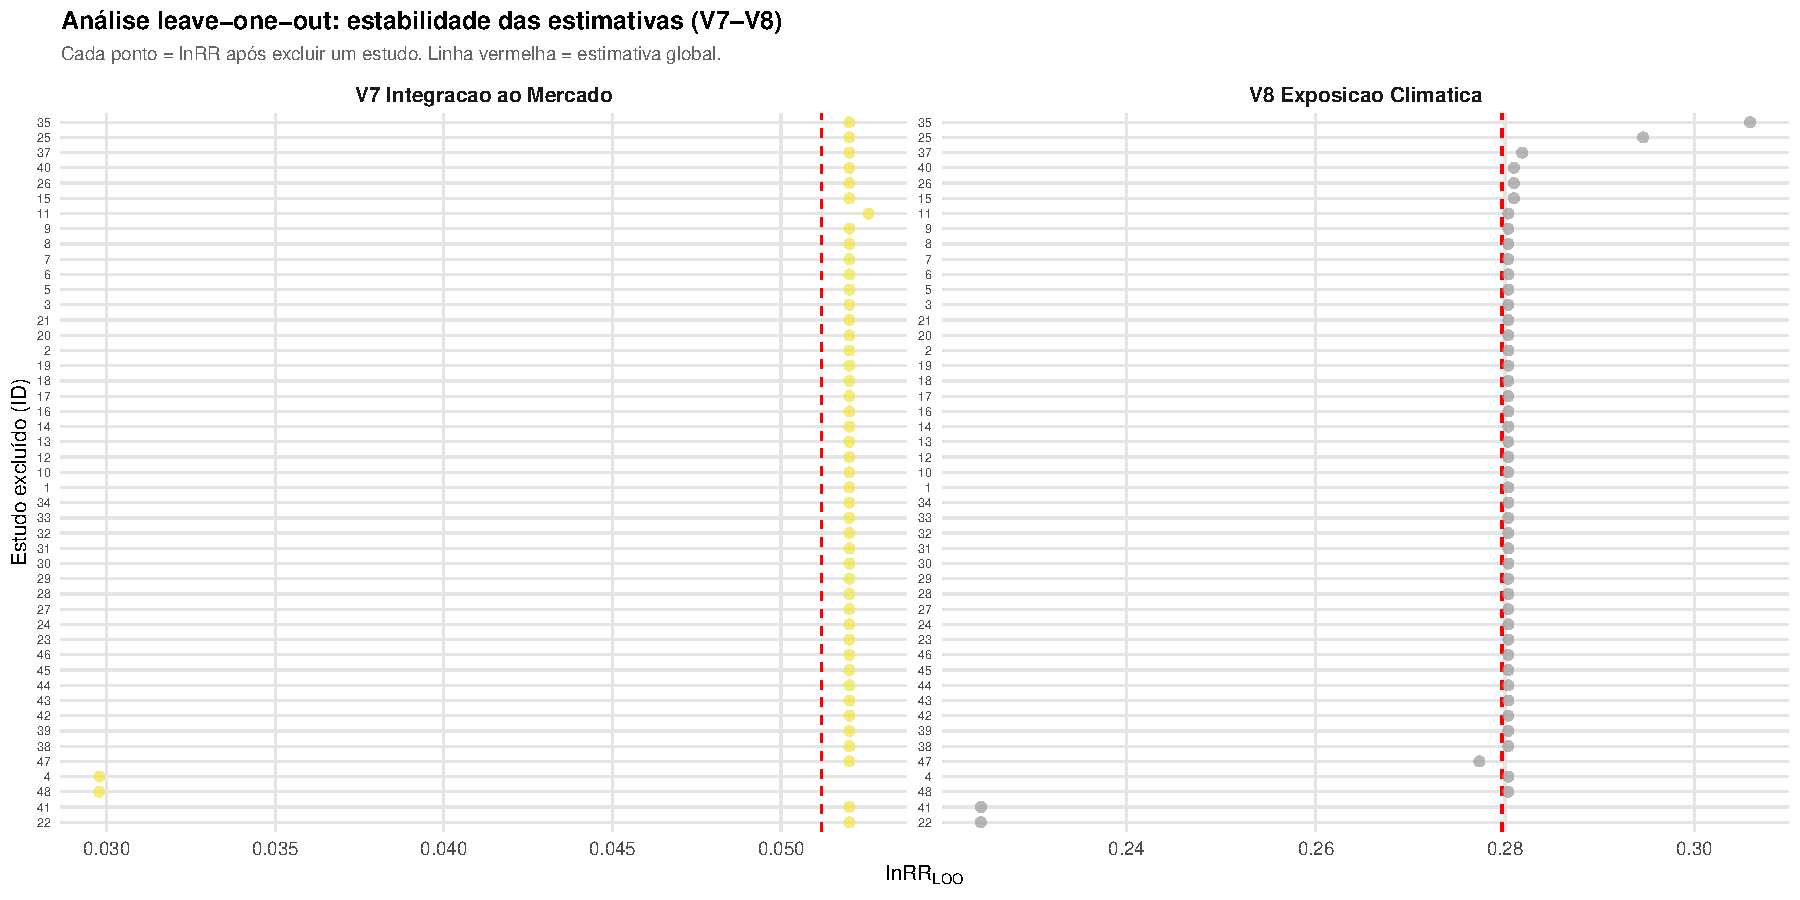
\includegraphics[width=\textwidth]{3-FIGURAS/leave_one_out_V7_V8.pdf}
  \caption{Dimensões $V_7$--$V_8$: integração ao mercado e exposição climática}
  \label{fig:loo-c}
\end{subfigure}
\caption{Análise \textit{leave-one-out}: estabilidade das estimativas de \texorpdfstring{$\overline{lnRR}$}{lnRR} após exclusão sequencial de cada estudo. (a) Dimensões $V_1$--$V_3$. (b) Dimensões $V_4$--$V_6$. (c) Dimensões $V_7$--$V_8$. A linha vermelha tracejada indica a estimativa global com todos os estudos incluídos}
\label{fig:loo}
\end{figure}

\subsection{O paradoxo da vulnerabilidade reconhecida mas não mensurada}
\label{sec:thematic-profile}

O corpus de 48 registros concentra-se em \textit{traditional knowledge}, \textit{biocultural diversity}, \textit{agrobiodiversity} e \textit{ethnobotany}, confirmando a adequação da filtragem PICOS à interseção entre conhecimento ecológico local e conservação. Essa coesão temática mascara, contudo, uma disjunção epistemológica, pois virtualmente todos os registros reconhecem ameaças aos saberes tradicionais \citep{Mobarak2025,LaRosa2021,Suwardi2025,Essien2025}, porém apenas 7 dos 48 (14,6\%) empregam ``vulnerabilidade'' como variável de investigação e somente \citet{Zeleke2025} operacionaliza o conceito com framework de 15 indicadores estruturados em exposição, sensibilidade e capacidade adaptativa. 

A proporção de 31 estudos qualitativos para 17 quantitativos (64,6\% vs.\ 35,4\%) confirma que a vulnerabilidade biocultural permanece metodologicamente suboperacionalizada, fenômeno atribuível a tradições etnográficas que tratam a quantificação com cautela por risco de descontextualização \citep{Agrawal2002}. Essa lacuna é particularmente relevante porque a taxonomia de ameaças ao conhecimento ecológico tradicional proposta por \citet{TangGavin2016} identifica vetores de pressão múltiplos e interativos cuja operacionalização demanda indicadores compostos, ao passo que o alerta científico de \citet{FernandezLlamazares2021} documenta a convergência global de ameaças sobre sistemas de conhecimento indígena sem oferecer métricas de mensuração padronizadas. A presente meta-análise busca preencher essa lacuna metodológica entre o acervo descritivo e a quantificação necessária para subsidiar decisões de salvaguarda.

\subsection{Erosão intergeracional como variável-nexo}
\label{sec:dimensional-coverage}

Dentre as oito dimensões de vulnerabilidade propostas ($V_1$--$V_8$), a erosão intergeracional ($V_1$) se distingue na leitura do corpus não como uma dimensão equivalente às demais, mas como o mecanismo pelo qual todas as outras se reproduzem ou colapsam. Doze dos 48 estudos documentam explicitamente processos de transferência de conhecimento, e a diversidade dos contextos investigados indica que a transmissão não é um ato singular, mas um sistema de práticas distribuídas que assume formas distintas dependendo do ecossistema, do gênero e da estrutura comunitária.

\citet{Cantor2025} demonstra que o conhecimento necessário para a pesca cooperativa com golfinhos na costa brasileira é transmitido por aprendizado situado, cuja ruptura implica não apenas perda de saber técnico, mas dissolução de uma relação interespecífica coevoluída. \citet{Sibanda2025} evidencia que a custódia feminina de sementes crioulas no Zimbabwe sustenta simultaneamente a soberania alimentar doméstica, a identidade cultural e a transmissão de conhecimento intergeracional, de modo que a vulnerabilidade seminal e a vulnerabilidade epistêmica são, nesse contexto, a mesma variável. \citet{Gerner2025} revela que a preservação de saberes sobre plantas medicinais na Europa depende de dinâmicas sociais comunitárias cujo enfraquecimento por migração desestrutura os mecanismos informais de transferência.

Esses estudos, em conjunto, indicam que a transmissão intergeracional não opera como dimensão estanque, mas como variável mediadora cuja falha pode precipitar o declínio das demais dimensões. Essa interpretação é consistente com evidências longitudinais de perda de conhecimento tradicional em sociedades contemporâneas \citep{ReyesGarcia2013evidence}, com a erosão documentada em contextos pastoris Maasai \citep{HedgesKipila2020} e entre os Tsimane' \citep{Gruberg2022}, sugerindo que o fenômeno transcende fronteiras geográficas e culturais. A co-ocorrência entre vetores de pressão exógena (migração, urbanização, integração de mercado) e erosão de saberes sustenta essa interpretação, na medida em que \citet{Tran2025} documenta como políticas de relocação no Vietnam desarticulam redes comunitárias de gestão hídrica tradicional, \citet{Moller2023} identifica a emigração como vetor primário de perda de saberes ecológicos em comunidades rurais sul-africanas, e \citet{Aniah2019} demonstra que a variabilidade climática no norte de Gana força a adoção de estratégias de subsistência alternativas que competem com a transmissão de práticas agrícolas tradicionais.

Essa centralidade funcional de $V_1$ tem implicação direta para a interpretação dos rankings de magnitude de efeito e para a eventual construção de instrumentos compostos de avaliação de vulnerabilidade. Se a erosão intergeracional opera como nexo causal entre pressões exógenas e o decaimento de todas as dimensões, tratá-la com peso simétrico às demais subestimaria sua contribuição real para a vulnerabilidade agregada, o que deve ser considerado em estudos subsequentes de modelagem. O efeito próximo de zero observado para $V_1$ ($\overline{lnRR} = -0{,}017$) não contradiz essa centralidade, pois reflete a contrabalancagem entre comunidades onde a transmissão é ativamente reforçada por intervenções de salvaguarda e comunidades onde o colapso já se instalou, cancelando o efeito agregado.

A dimensão de status de documentação ($V_3$) apresentou efeito próximo de zero ($\overline{lnRR} = +0{,}007$; $I^2 = 7{,}6\%$), porém a meta-regressão revelou coeficientes individuais que iluminam a dinâmica interna dessa dimensão. Indicadores de conhecimento ecológico apresentaram tendência positiva ($\beta = +0{,}513$; $p < 0{,}001$), capturando processos de registro formal onde inventários estruturados e protocolos de digitalização transformam conhecimento tácito em documentação auditável \citep{Zeleke2025,Suwardi2025}, ao passo que avaliações etnobotânicas ($\beta = -0{,}405$; $p < 0{,}001$), avaliações de agrobiodiversidade ($\beta = -0{,}405$; $p < 0{,}001$) e avaliações agroflorestais ($\beta = -1{,}078$; $p = 0{,}075$) sugeriram efeito protetor, indicando que abordagens holísticas de documentação preservam melhor as relações funcionais entre práticas, territórios e agentes de transmissão \citep{Maina2012,Poorna2014}. Iniciativas de preservação digital de sistemas de conhecimento indígena \citep{Balogun2021} reforçam que a documentação efetiva requer integração entre formatos audiovisuais, metadados contextuais e protocolos de governança comunitária.

A lacuna mais evidente do corpus reside na suboperacionalização da vulnerabilidade jurídica como variável de investigação. Embora $V_4$ concentre um dos dois efeitos significativos da síntese, nenhum dos 48 estudos primários emprega ``vulnerabilidade jurídica'' como variável explícita, descrevendo processos equivalentes sob terminologias fragmentadas como ``erosão da diversidade biocultural'' \citep{Mobarak2025}, ``perda de conhecimento local e indígena'' \citep{Suwardi2025} e ``desaparecimento da história oral'' \citep{LaRosa2021}. Essa dispersão terminológica sugere que uma dimensão empiricamente relevante permanece conceitualmente difusa, reforçando a necessidade de marcos analíticos unificados como o aqui proposto. A escassez de operacionalização é notável dado que a literatura existente sobre propriedade intelectual \citep{Dutfield2004} e jurisprudência biocultural \citep{BavikatteRobinson2011,Nemoga2022} já oferece caminhos teóricos e práticos para a mensuração da vulnerabilidade jurídica.

A exposição climática ($V_8$), segundo efeito significativo da síntese ($\overline{lnRR} = +0{,}280$; IC~95\%: $[0{,}03;\; 0{,}53]$), indica que comunidades submetidas a maior variabilidade pluviométrica e frequência de eventos extremos tendem a apresentar indicadores de vulnerabilidade biocultural 32,3\% superiores. A homogeneidade dessa estimativa ($I^2 \approx 0$; PI~95\%: $[0{,}04;\; 0{,}52]$) sugere que o efeito opera de forma consistente entre contextos geográficos e culturais distintos, diferindo do padrão regionalmente heterogêneo observado para $V_4$. Esse resultado é compatível com evidências de que perturbações climáticas forçam a substituição de calendários de cultivo tradicionais por estratégias de subsistência alternativas que competem diretamente com a transmissão de saberes agrícolas, promovem a perda de variedades locais adaptadas a regimes pluviométricos históricos \citep{Savo2016} e podem desarticular redes comunitárias de gestão hídrica cujo funcionamento depende de conhecimento ecológico contextual. A interação entre pressão climática e descontinuidade intergeracional reforça a interpretação de $V_1$ como variável mediadora, na medida em que a percepção de reduzida relevância prática dos saberes tradicionais sob regimes climáticos alterados pode acelerar o abandono da transmissão vertical. A integração ao mercado ($V_7$, $\overline{lnRR} = +0{,}051$) exibiu tendência marginal de 5,3\%, compatível com a hipótese de que a substituição progressiva de variedades crioulas por cultivares comerciais constitui vetor de erosão biocultural cuja magnitude, contudo, permanece inferior à da pressão climática e institucional no corpus analisado.

\subsection{Implicações para a avaliação de vulnerabilidade e direcionamento da extração}
\label{sec:vulnerability-implications}

Comunidades de agricultores sul-americanos apresentaram a maior vulnerabilidade jurídica ($\overline{lnRR} = -0{,}464$ para região, $-0{,}395$ para tipo de comunidade), sugerindo que intervenções de fortalecimento de regimes de tenure e registro patrimonial formal podem ser prioritárias nesses contextos. Estratégias ancoradas em territórios simbólicos (bosques sagrados, áreas cerimoniais) apresentaram os maiores coeficientes protetores ($\beta_{V5} = +1{,}496$; $\beta_{V6} = +1{,}407$), sugerindo que a articulação entre práticas rituais e visibilidade institucional pode produzir efeitos simultâneos sobre coesão social e vitalidade cultural, resultado compatível com a reconceptualização de conservação comunitária proposta por \citet{Berkes2004} e com a cogestão adaptativa como mecanismo de construção de resiliência \citep{OlssonFolkeBerkes2004}. A mitigação da exposição climática ($V_8$) constitui o quarto eixo, dado que a consistência do efeito entre contextos ($I^2 \approx 0$) sugere que a vulnerabilidade associada a eventos extremos opera como pressão transversal cuja resposta pode demandar a integração entre adaptação climática e salvaguarda de saberes tradicionais. Abordagens centradas exclusivamente em indicadores ecológicos isolados ($\beta_{V5} = -0{,}919$) não apenas não se associaram a efeitos protetores, mas podem ter capturado processos de erosão já em andamento.

A composição metodológica do corpus (64,6\% de estudos qualitativos) reflete uma tensão epistemológica constitutiva do campo, na qual a quantificação de saberes tácitos e relacionais enfrenta objeções legítimas quanto a reificação \citep{Agrawal2002,GomezBaggethun2013}. A estratégia adotada nesta meta-análise responde parcialmente a essa tensão ao ancorar as estimativas em razões de resposta com propagação explícita de incerteza e ao manter $I^2$ como parâmetro de cautela interpretativa.

A identificação de gênero como tema transversal em oito estudos (16,7\%) sugere que esse moderador pode ser relevante para a compreensão da vulnerabilidade biocultural e merece investigação em meta-regressões futuras. \citet{RomeroSilva2026} documenta o papel de mulheres na conservação de agrobiodiversidade em \textit{homegardens} mesoamericanos, e \citet{MugiNgenga2016} identifica assimetrias de gênero na intensificação agrícola, sinalizando que comunidades com maior participação feminina na governança de saberes podem apresentar magnitudes de efeito distintas em $V_1$ (erosão intergeracional) e $V_3$ (status de documentação).


\subsection{Moderadores e estabilidade das estimativas}
\label{sec:moderadores-discussao}

América do Sul e Ásia concentram os efeitos negativos significativos para $V_4$ (Fig.~\ref{fig:meta-reg-regiao}), configurando um gradiente continental de vulnerabilidade jurídica consistente com contextos onde a pressão fundiária sobre territórios tradicionais se conjuga com fragilidade institucional, acelerando a erosão dos marcos jurídicos de proteção. Nas regiões africana e europeia, contudo, os intervalos de confiança permanecem compatíveis com neutralidade, sugerindo que fatores protetores regionais operam como \textit{buffers} contra a erosão documental. No Zimbabwe, a custódia comunitária de sementes documentada por \citet{Sibanda2025} exemplifica esse mecanismo compensatório, enquanto as redes etnobotânicas europeias descritas por \citet{Gerner2025} representam estruturas de salvaguarda funcionalmente análogas. A resiliência de sistemas de conhecimento agrícola em \textit{home gardens} ibéricos \citep{ReyesGarcia2014} e a integração de saberes contéxto-específicos na recuperação de espécies culturalmente significativas \citep{Rayne2022} ilustram como a complexidade biocultural ($V_2$) pode operar como fator protetor quando preservada. Essa assimetria geográfica sugere que políticas de proteção podem beneficiar-se de calibração regional, priorizando a América Latina e o Sudeste Asiático.

Comunidades de agricultores tradicionais apresentam a maior fragilidade jurídica ($\overline{lnRR} = -0{,}395$, Fig.~\ref{fig:meta-reg-comunidade}), superando tanto comunidades indígenas ($\overline{lnRR} = -0{,}241$) quanto rurais ($\overline{lnRR} = -0{,}156$). Essa diferença sugere que os mecanismos de proteção legal disponíveis para povos indígenas, incluindo marcos regulatórios de propriedade intelectual e protocolos de Nagoya \citep{BavikatteRobinson2011,Robinson2014}, proporcionam proteção parcial que não alcança comunidades de agricultores tradicionais sem reconhecimento étnico-territorial formal. Em contraste, a tendência positiva de $V_5$ em comunidades rurais ($\overline{lnRR} = +0{,}688$), embora sem significância estatística, aponta para a organização coletiva como possível mecanismo compensatório diante da vulnerabilidade em outras dimensões, resultado compatível com a hipótese de que a aprendizagem social e a evolução de práticas de conservação dependem de redes de governança adaptativa \citep{BerkesTurner2006,Folke2004}.

Intervenções ancoradas em territórios simbólicos, como a conservação de bosques sagrados (Fig.~\ref{fig:meta-reg-intervencao}), emergiram como o moderador com maior efeito protetor simultâneo em $V_5$ ($\beta = +1{,}496$; $p = 0{,}014$) e $V_6$ ($\beta = +1{,}407$; $p = 0{,}001$), indicando que práticas territorialmente enraizadas podem produzir efeitos sinérgicos sobre coesão social e vitalidade cultural. Indicadores de conhecimento ecológico, em contrapartida, apresentaram efeito negativo em $V_5$ ($\beta = -0{,}919$; $p < 0{,}001$), sugerindo que esse tipo de mensuração pode capturar processos erosivos já em andamento. Esses contrastes reforçam a necessidade de distinguir entre intervenções \textit{ex situ}, focadas em monitoramento e catalogação, e intervenções \textit{in situ}, voltadas ao fortalecimento de práticas territoriais \citep{Zimmerer2018}, na formulação de estratégias de salvaguarda. A interdependência entre extinção linguística e perda de conhecimento medicinal único \citep{CamaraLeret2021} reforça que a complexidade biocultural ($V_2$) não pode ser avaliada isoladamente das dimensões de organização social e vitalidade linguística.

Nenhuma exclusão individual reverteu a direção ou a significância dos efeitos nas oito dimensões (Fig.~\ref{fig:loo}). Para $V_4$ (vulnerabilidade jurídica), nenhuma exclusão individual reverteu a direção do efeito negativo ($\Delta_{\max} = 0{,}075$), e a remoção de \citet{Sibanda2025}, estudo com maior peso amostral, aprofundou a estimativa de $-0{,}279$ para $-0{,}354$, o que indica que o resultado não depende de um único estudo influente. Para $V_3$ (status de documentação), a maior sensibilidade observada ($\Delta_{\max} = 0{,}077$) permaneceu modesta em relação ao efeito próximo de zero, sem alterar a direção da estimativa. Para $V_2$ (complexidade biocultural), a baixa sensibilidade à exclusão ($\Delta_{\max} = 0{,}028$) alinha-se com a baixa heterogeneidade ($I^2 = 3{,}6\%$), indicando a dimensão com efeito mais homogeneamente distribuído entre os estudos.

\subsection{Limitações}
\label{sec:limitations}

Considerando a natureza meta-analítica desta pesquisa, é pertinente reconhecer algumas limitações. Uma delas refere-se à predominância de evidência qualitativa no corpus (74,5\% dos registros classificados como Tier~3 ou Tier~4), o que significa que a maioria dos tamanhos de efeito deriva de conversões ordinais; todavia, a inflação de variância aplicada por tier foi desenhada para acomodar essa incerteza, e os resultados permaneceram estáveis na análise de sensibilidade. Outra possível limitação diz respeito aos tamanhos amostrais reduzidos em algumas estratificações por região e tipo de comunidade ($k = 1$--$12$), o que pode restringir a transferência dos achados para contextos não representados. Ainda assim, os padrões observados são consistentes com a literatura e oferecem base para a formulação de hipóteses em investigações futuras.


%% ============================================================
%% 5. CONCLUSÃO
%% ============================================================
\section{Conclusão}
\label{sec:conclusions}

Os resultados indicam que a fragilidade institucional, operacionalizada pela vulnerabilidade jurídica e fundiária ($V_4$), e a exposição climática ($V_8$) constituem os dois vetores significativos de degradação biocultural em saberes e sistemas agrícolas tradicionais, ao passo que indicadores ecológicos, de documentação e de complexidade biocultural apresentaram efeitos próximos de zero. A vulnerabilidade jurídica concentrou-se em comunidades de agricultores tradicionais sul-americanos, onde a desconexão entre regimes consuetudinários de posse e marcos regulatórios nacionais acentua a erosão dos mecanismos de proteção, enquanto a exposição climática operou de forma homogênea entre contextos geográficos e culturais, sugerindo que a pressão de eventos extremos constitui vetor transversal de degradação. A transmissão intergeracional ($V_1$) opera como variável mediadora cuja falha pode precipitar o declínio simultâneo das demais dimensões, sinalizando que a continuidade desses sistemas depende mais da manutenção das condições jurídicas, territoriais e sociais do que do volume de saberes documentados. Intervenções ancoradas em territórios simbólicos apresentaram os maiores coeficientes protetores simultâneos sobre organização social ($V_5$) e vitalidade linguística ($V_6$), indicando que políticas de salvaguarda podem beneficiar-se da articulação entre reforço jurídico-fundiário, fortalecimento da organização comunitária e adaptação climática.

%% ============================================================
%% Agradecimentos
%% ============================================================
\section*{Agradecimentos}

Os autores agradecem ao Programa de Pós-Graduação em Ciências da Propriedade Intelectual (PPGPI/UFS) pelo apoio institucional. Este estudo contou com suporte do Conselho Nacional de Desenvolvimento Científico e Tecnológico (CNPq) e da Fundação de Amparo à Pesquisa do Estado da Bahia (FAPESB).


%% ============================================================
%% MATERIAL SUPLEMENTAR
%% ============================================================
\section*{Material Suplementar}

O Material Suplementar associado a este artigo pode ser encontrado na versão online em [DOI a ser inserido]. O documento contém: Online Resource~1 -- Diagrama de fluxo PRISMA detalhando o processo de seleção de estudos; Online Resource~2 -- Tabela de resultados da meta-análise por dimensão de vulnerabilidade biocultural ($k = 37$--$47$ estudos, modelo \texttt{rma.mv} com REML e RVE-CR2, $\rho = 0{,}8$), incluindo intervalos de predição; Online Resource~3 -- Tabela de mapeamento entre indicadores meta-analíticos e dimensões funcionais; Online Resource~4 -- Tabela de diagnóstico de viabilidade por dimensão.

%% ============================================================
%% REFERÊNCIAS
%% ============================================================
\bibliographystyle{plainnat}    %% natbib autor-ano (compatível com Springer)
\bibliography{references}


%% ============================================================
%% DECLARAÇÕES (após referências, conforme diretrizes B&C)
%% ============================================================
\section*{Statements and Declarations}

\subsection*{Funding}

O presente trabalho foi realizado com apoio da Coordenação de Aperfeiçoamento de Pessoal de Nível Superior -- Brasil (CAPES).

\subsection*{Competing Interests}

Os autores declaram não possuir conflitos de interesse financeiros ou relações pessoais conhecidas que possam ter influenciado o trabalho relatado neste artigo.

\subsection*{Author Contributions}

\textbf{Catuxe Varjão de Santana Oliveira:} Conceituação, Metodologia, Investigação, Análise formal, Curadoria de dados, Escrita -- rascunho original. \textbf{Luiz Diego Vidal Santos:} Metodologia, Análise formal, Validação, Escrita -- revisão e edição.
\textbf{Paulo Roberto Gagliardi:} Escrita -- revisão e edição, Supervisão.
\textbf{Tânia Cristina Azevedo:} Escrita -- revisão e edição.
\textbf{Renisson Neponuceno de Araújo Filho:} Escrita -- revisão e edição.
\textbf{Francisco Sandro Rodrigues Holanda:} Escrita -- revisão e edição.

\subsection*{Data Availability}

O dataset de extração, os scripts de análise e os outputs meta-analíticos estão disponíveis no Mendeley Data (\url{https://doi.org/10.17632/mh5sbx7ky7.1}).

\end{document}
